%%%%%%%%%%%%%%%%%%%%%%%%%%%%%%%%%%%%%%%%%%%%%%%%%%%%%%%%%%%%%%%%%%%%%%%%%%%%%%%%%%%%%%%%%%%%%%%%%%%%%%%%%%%%%%%%%%%%%%%%%%%%%%%%%%%%%%%%%%%%%
\section{Phase imprinting defects}\label{sec:phase}
%%%%%%%%%%%%%%%%%%%%%%%%%%%%%%%%%%%%%%%%%%%%%%%%%%%%%%%%%%%%%%%%%%%%%%%%%%%%%%%%%%%%%%%%%%%%%%%%%%%%%%%%%%%%%%%%%%%%%%%%%%%%%%%%%%%%%%%%%%%%%

Where previously I added an optical potential to the Hamiltonian for a short time during the evolution, here I directly engineer the wavefunction phase. For the previously chosen kicking strengths and timestep, the limiting values of the phase change are $\approx 0.2 < \phi < \approx 0.94$. This is determined by writing the phase as
\begin{equation}
    e^{i\phi} \mapsto \exp\left(-i\frac{V_{\textrm{opt}}dt}{\hbar}\right),
\end{equation}
and filling in for the defined simulation values. Thus, for a much stronger phase change a longer lasting pulse, or a greater amplitude are two possible contenders. However, as discussed previously, neither are suitable candidates in this system, given the lattice rotation, as well as the excitation of higher-order wavenumbers. With the use of direct phase imprinting we can realise arbitrary phase patterns on the condensate. Previously the vortex lattice was unaffected by the imprint; here I attempt to destroy the vortex lattice by directly engineering the opposite phase winding profile atop a lattice vortex. This has the distinct advantage of locally erasing a vortex and disordering the lattice. I will now discuss this method.

Phase imprinting is a technique that applies a spatially inhomogeneous optical potential across a condensate in such a way that the phase is modified to a desired form. As a consequence the density distribution will adjust itself and in ground state condensates dark solitons \cite{BEC:Denschlag_science_2000}, as well as vortices \cite{Vtx:Dobrek_pra_1999} have been created this way. For the latter the signature is given by a phase singularity, around which the phase winds through $\pm 2\pi$, depending upon the direction of rotation.

The phase imprinting method can also be used to annihilate a vortex from the lattice by applying a phase profile of opposite winding, removing the phase singularity.  This will leave the condensate with a density depletion at the prior location of the phase singularity. Without the singularity this depletion will fill in and excite phonon modes in the condensate during time evolution. This method will form the basis for which the further discussions and analysis are performed on the vortex carrying condensate.


%%%%%%%%%%%%%%%%%%%%%%%%%%%%%%%%%%%%%%%%%%%%%%%%%%%%%%%%%%%%%%%%%%%%%%%%%%%%%%%%%%%%%%%%%%%%%%%%%%%%%%%%%%%%%%%%%%%%%%%%%%%%%%%%%%%%%%%%%%%%%
\section{Model}\label{sec:model}
%%%%%%%%%%%%%%%%%%%%%%%%%%%%%%%%%%%%%%%%%%%%%%%%%%%%%%%%%%%%%%%%%%%%%%%%%%%%%%%%%%%%%%%%%%%%%%%%%%%%%%%%%%%%%%%%%%%%%%%%%%%%%%%%%%%%%%%%%%%%%

To investigate the evolution of a perturbed vortex lattice we numerically solve the Gross--Pitaevskii equation in two dimensions, assuming a strong confinement along the third axis. This allows to restrict the dynamics to the $x$--$y$ plane and focus fully on the Abrikosov lattice geometry. Experimental setups in lower dimensions are currently available \cite{BEC:Stock_lpl_2004,BEC:Seo_jkps_2014,BEC:Chomaz_natcom_2015} and in the frame co-rotating with the condensate, the non-linear mean field equation governing the BEC wave-function is given by
\begin{align}
i\hbar\partial_t \Psi(\mathbf{r},t) = \Big[&-\frac{\hbar^2}{2m}\nabla^2 + V\left(\mathbf{x}\right) \nonumber\\
&+ g\vert \Psi(\mathbf{r},t) \vert^2- \Omega L_z \Big]\Psi(\mathbf{r},t)
\end{align}
Here $V\left(\mathbf{x}\right)$ is the trapping geometry, $\Omega$ is the trap rotation frequency, and $L_z$ is the angular momentum operator along the $z$-direction. For the rapidly rotating case, the vortices form an ordered triangular lattice, that rotates equivalently to a solid-body in the large number limit. Simulating a large vortex lattice is a difficult numerical problem, due to the required grid size to resolve all aspects of the system both in position and momentum space. Thus, an advanced numerical technique is required to obtain solutions in a reasonable timescale. We have developed and made use of ``GPUE'' \cite{GPUEDOI}, an open-sourced, graphics processing unit (GPU) enabled Gross--Pitaevskii equation solver. This software allows for the solution of dynamical behaviours of linear and non-linear Schr\"odinger systems in significantly shorter times than alternative implementations \cite{AO:Morgan_pra_2013,Wittekblog_2016}.

%\subsection{Lattice order}

From the vortex lattice groundstate wavefunction we consider each individual vortex as an effective particle. As the unperturbed lattice is well ordered near the condensate center at timescales of up to several seconds we restrict our analysis therein. Given the coordinate locations for each individual vortex it is possible to calculate statistical quantities on the quality of the resulting lattice. Each vortex position was found by summing over adjacent grid sites, and looking for a $2\pi$ phase winding. This gave a vortex position estimated to the numerical grid. A least-squares fit was then performed to more accurately determine the vortex core to sub-grid resolution.

As we have an inhomogeneous density profile due to the harmonic confinement, and a system with a finite size, the use of translational correlations does not make much sense. Orientational correlations however, which measure how the lattice aligns along a particular angle may be useful. We calculate the orientational correlation function as
\begin{equation}
	g_6(r) = \frac{1}{N(r)}\displaystyle\sum\limits_{i,j}^{N(r)}\psi_6(\mathbf{r}_i)\psi_6^{*}(\mathbf{r}_j),
\end{equation}
with
\begin{equation}
	\psi_6(|\mathbf{r}_{i} - \mathbf{r}_{j}|) = \frac{1}{n_i}\displaystyle\sum\limits_j^{n_i}\exp(6\mathrm{i}(\theta_i - \theta_j)),
\end{equation}
where $\psi_6$ is the orientational order parameter, and $j$ is over the nearest neighbouring vortices.

We examine the orientational correlation function as a measure of the order of a ``vortex unit cell'', consisting of the angle made by nearest neighbours to an individual vortex. For a perfectly ordered triangular lattice this value will tend to 1. To maintain constant vortex areal density, we choose vortices defined at a radius of up to $r=2\times 10^{-4}$ m from the centre, which give an almost uniform lattice constant for our system parameters.

Additionally, we make use of the Delaunay triangulation of the vortex lattice to determine the occurrence of topological defects within the lattice. Delaunay triangulation generates a mesh from the vortex positions, wherein we examine the resulting triangulation for the appearance of non 6-fold connected vortices. When combined with other defects, such as a paired 5 and 7-fold connected vortex, these form dislocations in the crystal structure. These structures are countable, allowing us to directly determine the effect a perturbation has on the lattice.

\subsection{Few vortex dynamics}

To fully understand the effect of removing a vortex from the lattice system, let us first investigate the effects from removing the vorticity from a single vortex carrying condensate. Since the presence of vorticity requires the presence of a phase singularity, vortices possess the characteristic density depletion in their centre, which becomes unstable once the angular momentum is removed. The results of such a process can be seen in Fig.~\ref{fig:annihilation_1vtx}, and, as expected, the depletion of the condensate density fills in after the vortex phase is removed. An examination of the squared-radial expectation value, $\langle r^2 \rangle$, where $r^2 = x^2 + y^2$, shows that removing the vortex from the condensate excites a breathing mode, at the expected frequency of $2\omega_\perp$ for a two-dimensional system. The change in energy of the condensate is shown via the ratio of compressible (phonon) and incompressible (vortex) kinetic energy spectra given by Fig.~\ref{fig:kinspec}. As the vortex is annihilated we see a drop in the ratio of energies to favor a lower incompressible-to-compressible values for higher wavenumbers, resulting from the creation of a sound wave.

\begin{figure} \centering
    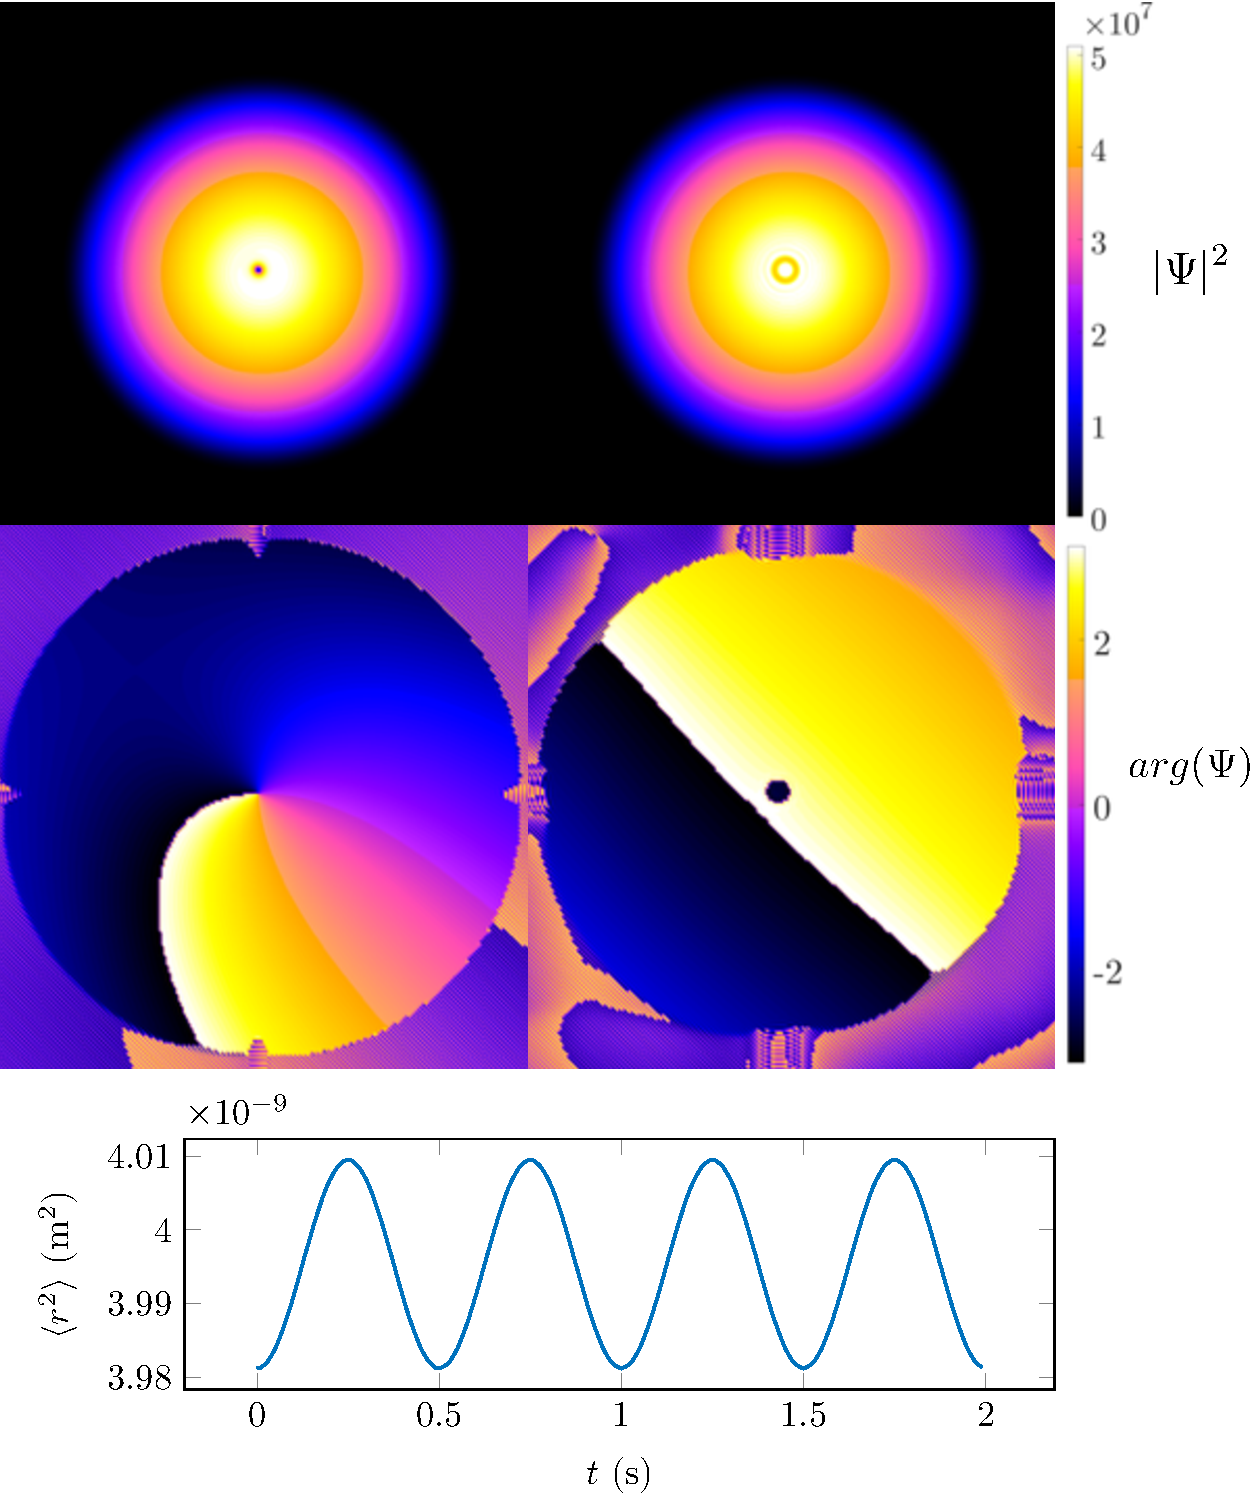
\includegraphics[width=0.55\textwidth]{ch6_phasegineer/imgs/NEWPICS/1vtx_remove1_centred2}
    \caption{The evolution of the condensate density and phase is shown for the initial state, and after 10 ms of evolution. The application of the phase creates sound waves which expand radially from the point of application. The line-plot shows the squared-radial expectation value which indicates the excitation of a breathing mode at $\omega_B = 2\omega_\perp$.}\label{fig:annihilation_1vtx}
\end{figure}

\begin{figure} \centering
    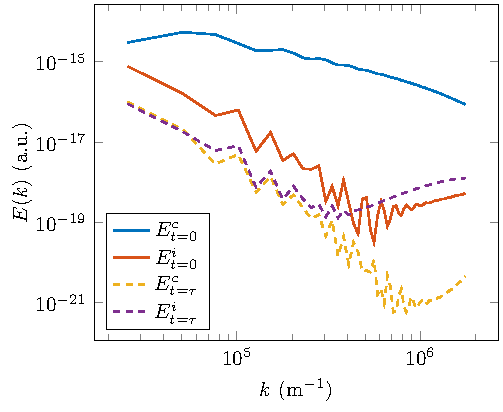
\includegraphics[width=0.55\textwidth]{ch6_phasegineer/tikz/EKt}
    \caption{The ratio of incompressible to compressible energies at times $t=0$ (solid) and $t=\tau$ (dashed), where $\tau=10$ ms. Initially the incompressible energy is greater than the compressible due to the presence of a vortex giving values greater than unity for all $k$. After application of the phase profile, the vortex is annihilated, with the energy released as phonons, indicated by a decrease in incompressible energy for higher $k$ values.}\label{fig:kinspec}
\end{figure}

\begin{figure} \centering
    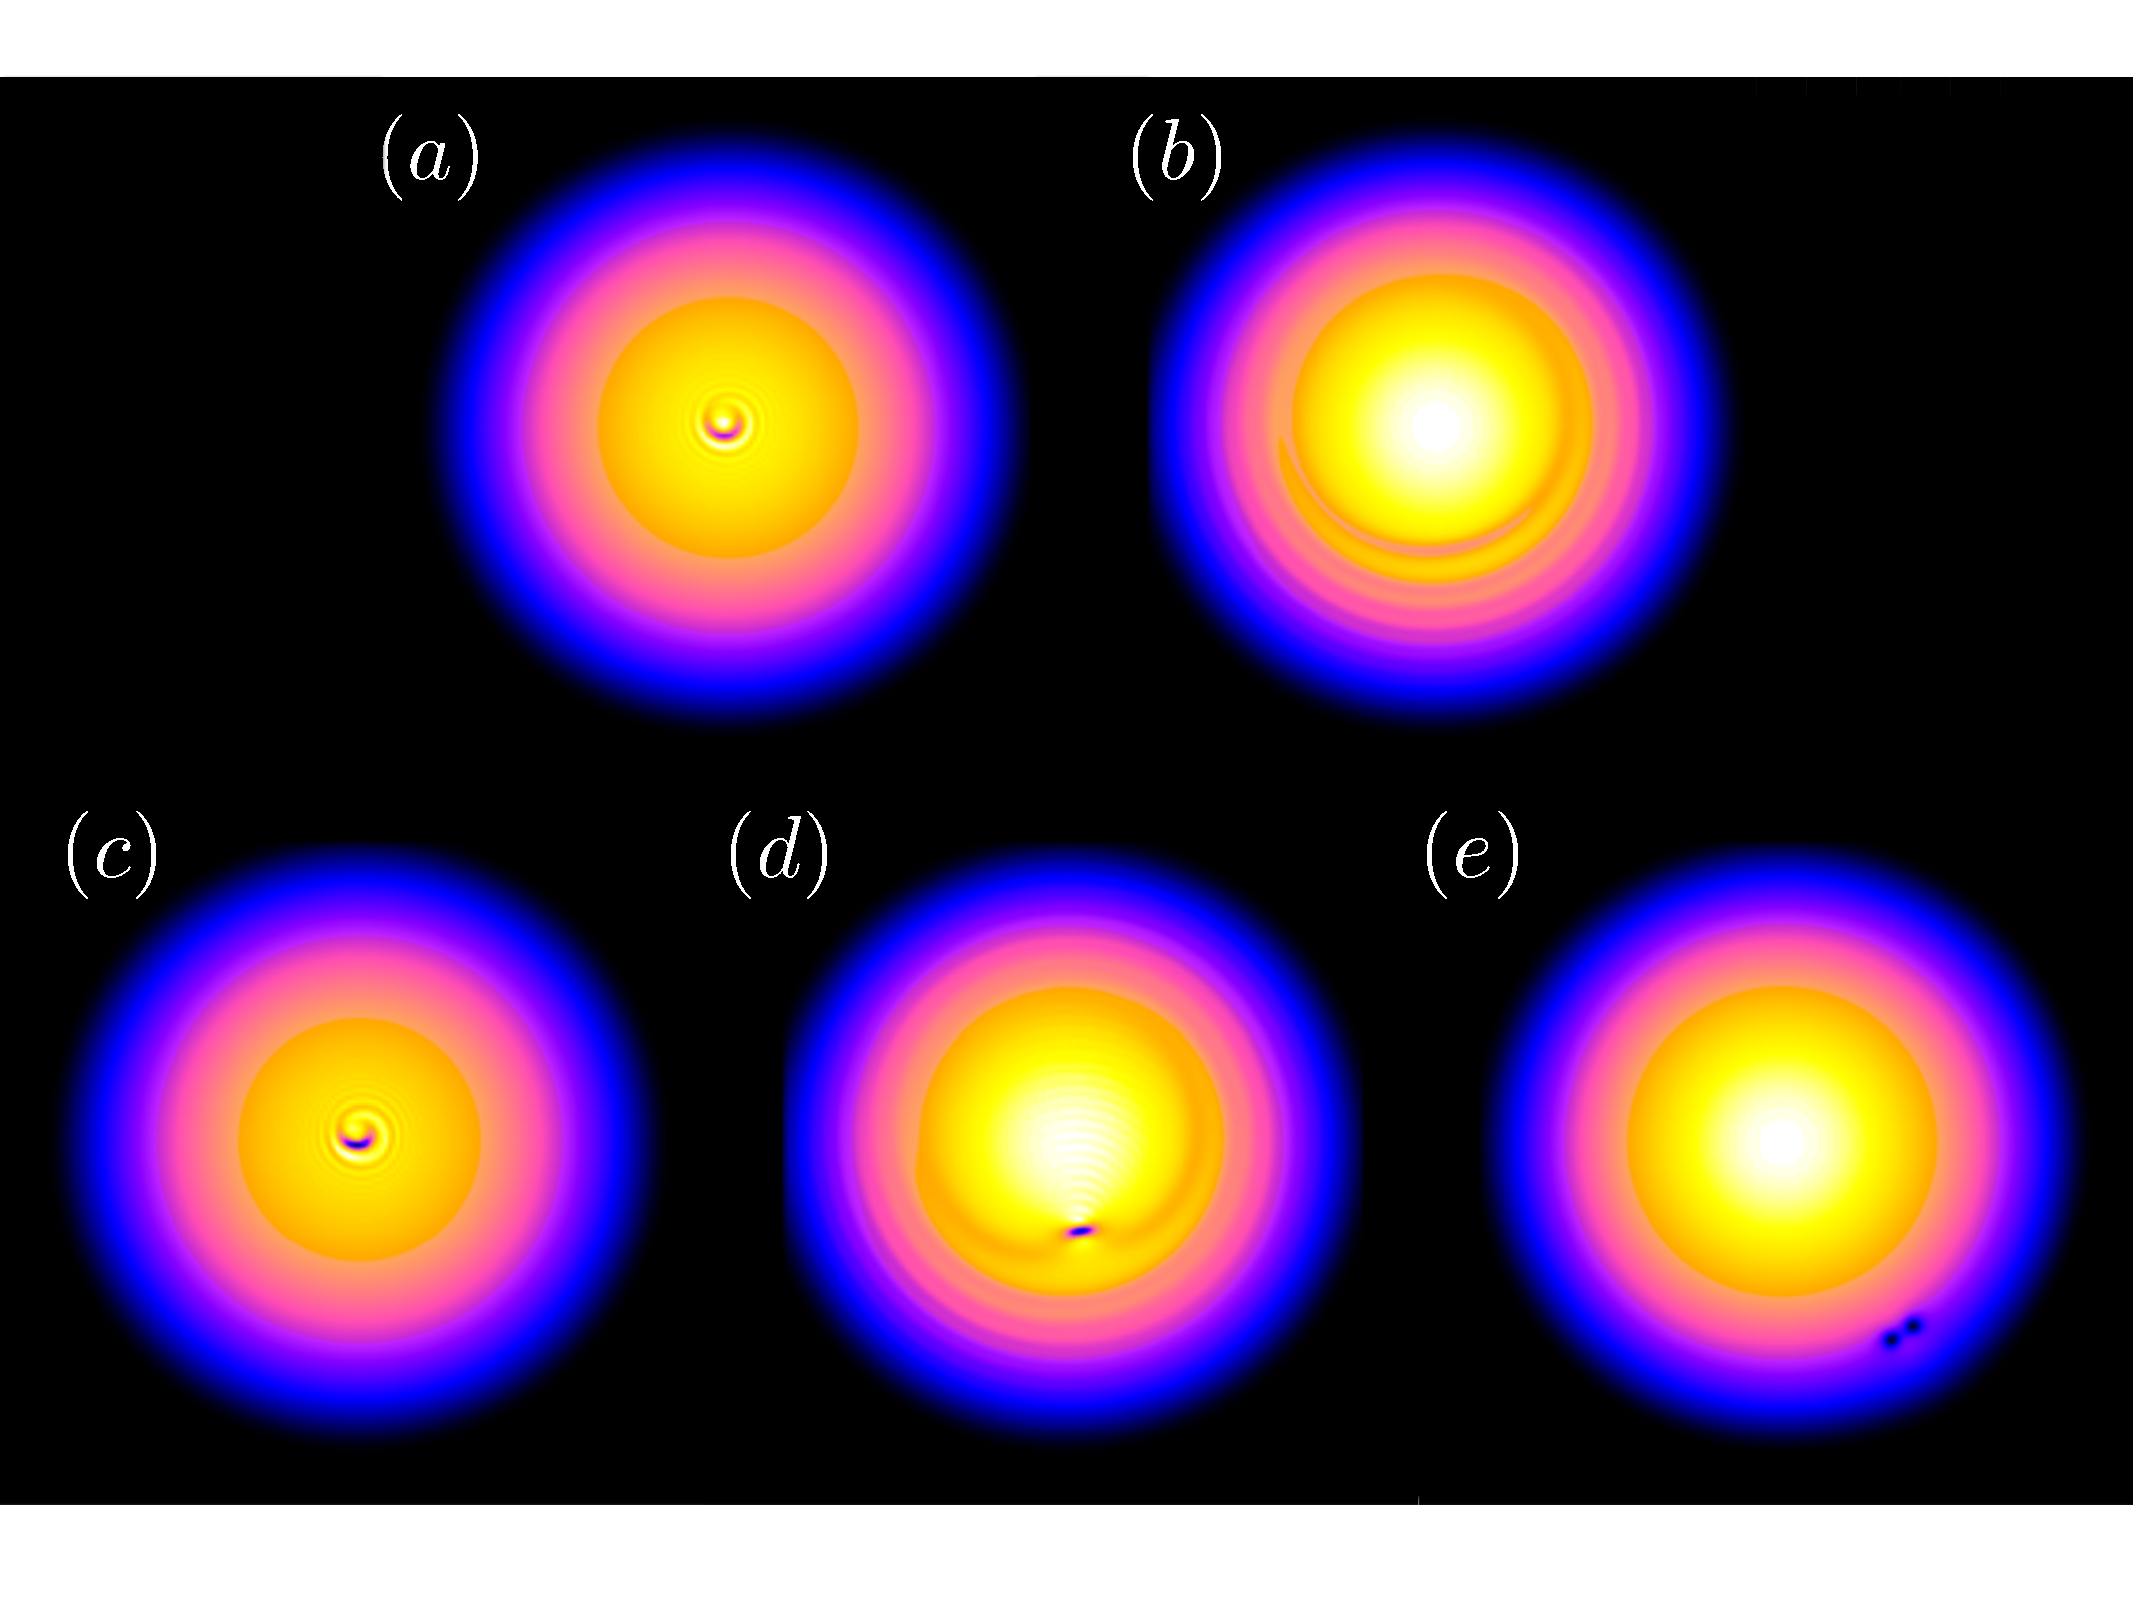
\includegraphics[width=0.55\textwidth]{ch6_phasegineer/imgs/1vtx_remove1_uncentred}
    \caption{The condensate evolution following an uncentered phase imprint. For an imprint that is of the order of the healing length from centre to centre, the annihilation occurs during the evolution (a,b). However, beyond this distance, we create an antivortex which travels with the pre-existing vortex and circulates the condensate (c,d,e).}\label{fig:annihilation_1vtx_uncentred}
\end{figure}

While the above suggest that erasing vortices is a straightforward and controllable process, this assumption needs to be checked for the situation where the imprinted phase and the exiting phase are not perfectly centered on each other.
%In addition to the ideal situation of perfect erasing of a centered vortex as discussed above, an additional situation is of interest: what happens when the erasing phase is not centred on the phase singularity (see Fig.~\ref{fig:annihilation_1vtx_uncentred}).
%As one can see
This situation is shown in Fig.~\ref{fig:annihilation_1vtx_uncentred} and one finds that cases where the imprinted profile is sufficiently close to the core (i.e. within a healing length) the existing vortex gets erased as before. However, beyond this distance a separate anti-vortex gets created and the vortex-antivortex pair travel to the edge of the condensate system, and begin to circulate around, as expected. For a densely packed lattice of vortices, this is not expected to be problematic given the expected proximity to additional cores following an imprint. %It is also worth noting all other vortices in the lattice away from the singularity should see a constant shift in phase, and thus remain largely unaffected.

As we have examined single vortex condensates, it is instructive to investigate the effect removal has on a single vortex in a two-vortex condensate. For this in Fig.~\ref{fig:2k1} we show a simulation where one vortex is erased in a two vortex condensate. One can see that the other vortex is no longer stationary in the corotating frame due to the change of the velocity field. This can be attributed to the condensate experiencing a constant shift in energy, with the vorticity of the remaining vortex unaffected. We verify this evaluating the condensate energy functional,
\begin{align}
    E(\Psi) = \int d\mathbf{r} \biggl( \frac{\hbar^2}{2m}|\nabla\Psi|^2 &+  \frac{1}{2}m\omega_\perp^2r^2|\Psi|^2 \nonumber\\ + \frac{g|\Psi|^4}{2} &- i\hbar\Omega\Psi^{*}(x\partial_y - y\partial_x)\Psi \biggr)
\end{align}
 for single vortex, two vortex, and two-less-one vortex condensates. This gives an energy hierarchy as $E_1 < E_{2-1} < E_2$, as expected, where $E_{2-1}-E_1\approx1.5$ and $E_2-E_{2-1}\approx 0.5$ in units of $\hbar\Omega$.

Although we have globally affected the angular momentum of the system, the other vortex remains on the same trajectory as before. The loss of the velocity field does not seem to disturb the vortex behaviour, other than the lack of stationarity in the co-rotating frame.

\subsection{Lattice dynamics}

%%%%%%%%%%%%%%%%%%%%%%%%%%%%%%%%%%%%%%%%%%%%%%%%%%%%%%%%%%%%%%%%%%%%%%%%%%%%%%%%%%%%%%%%%%%%%%%%%%%%%%%%%%%%%%%%%%%%%%%%%%%%%%%%%%%%%%%%%%%%%
The removal of a single vortex from the vortex lattice is expected to affect only the nearest neighbours by altering their velocity profile, with the overall angular momentum of the condensate decremented by a single quantum. Since phonons have been shown to yield minimal impact on the vortex lattice structure \cite{VTX:oriordan_pra_2016}, we can safely ignore their contribution from the phase imprint and annihilation. To examine the vortex dynamics following the application of the phase profile, each individual vortex is tracked independently. We can observe the local effects of disturbing the lattice by examining trajectory plots and the Delaunay triangulation of the vortex lattice.

\begin{figure}
    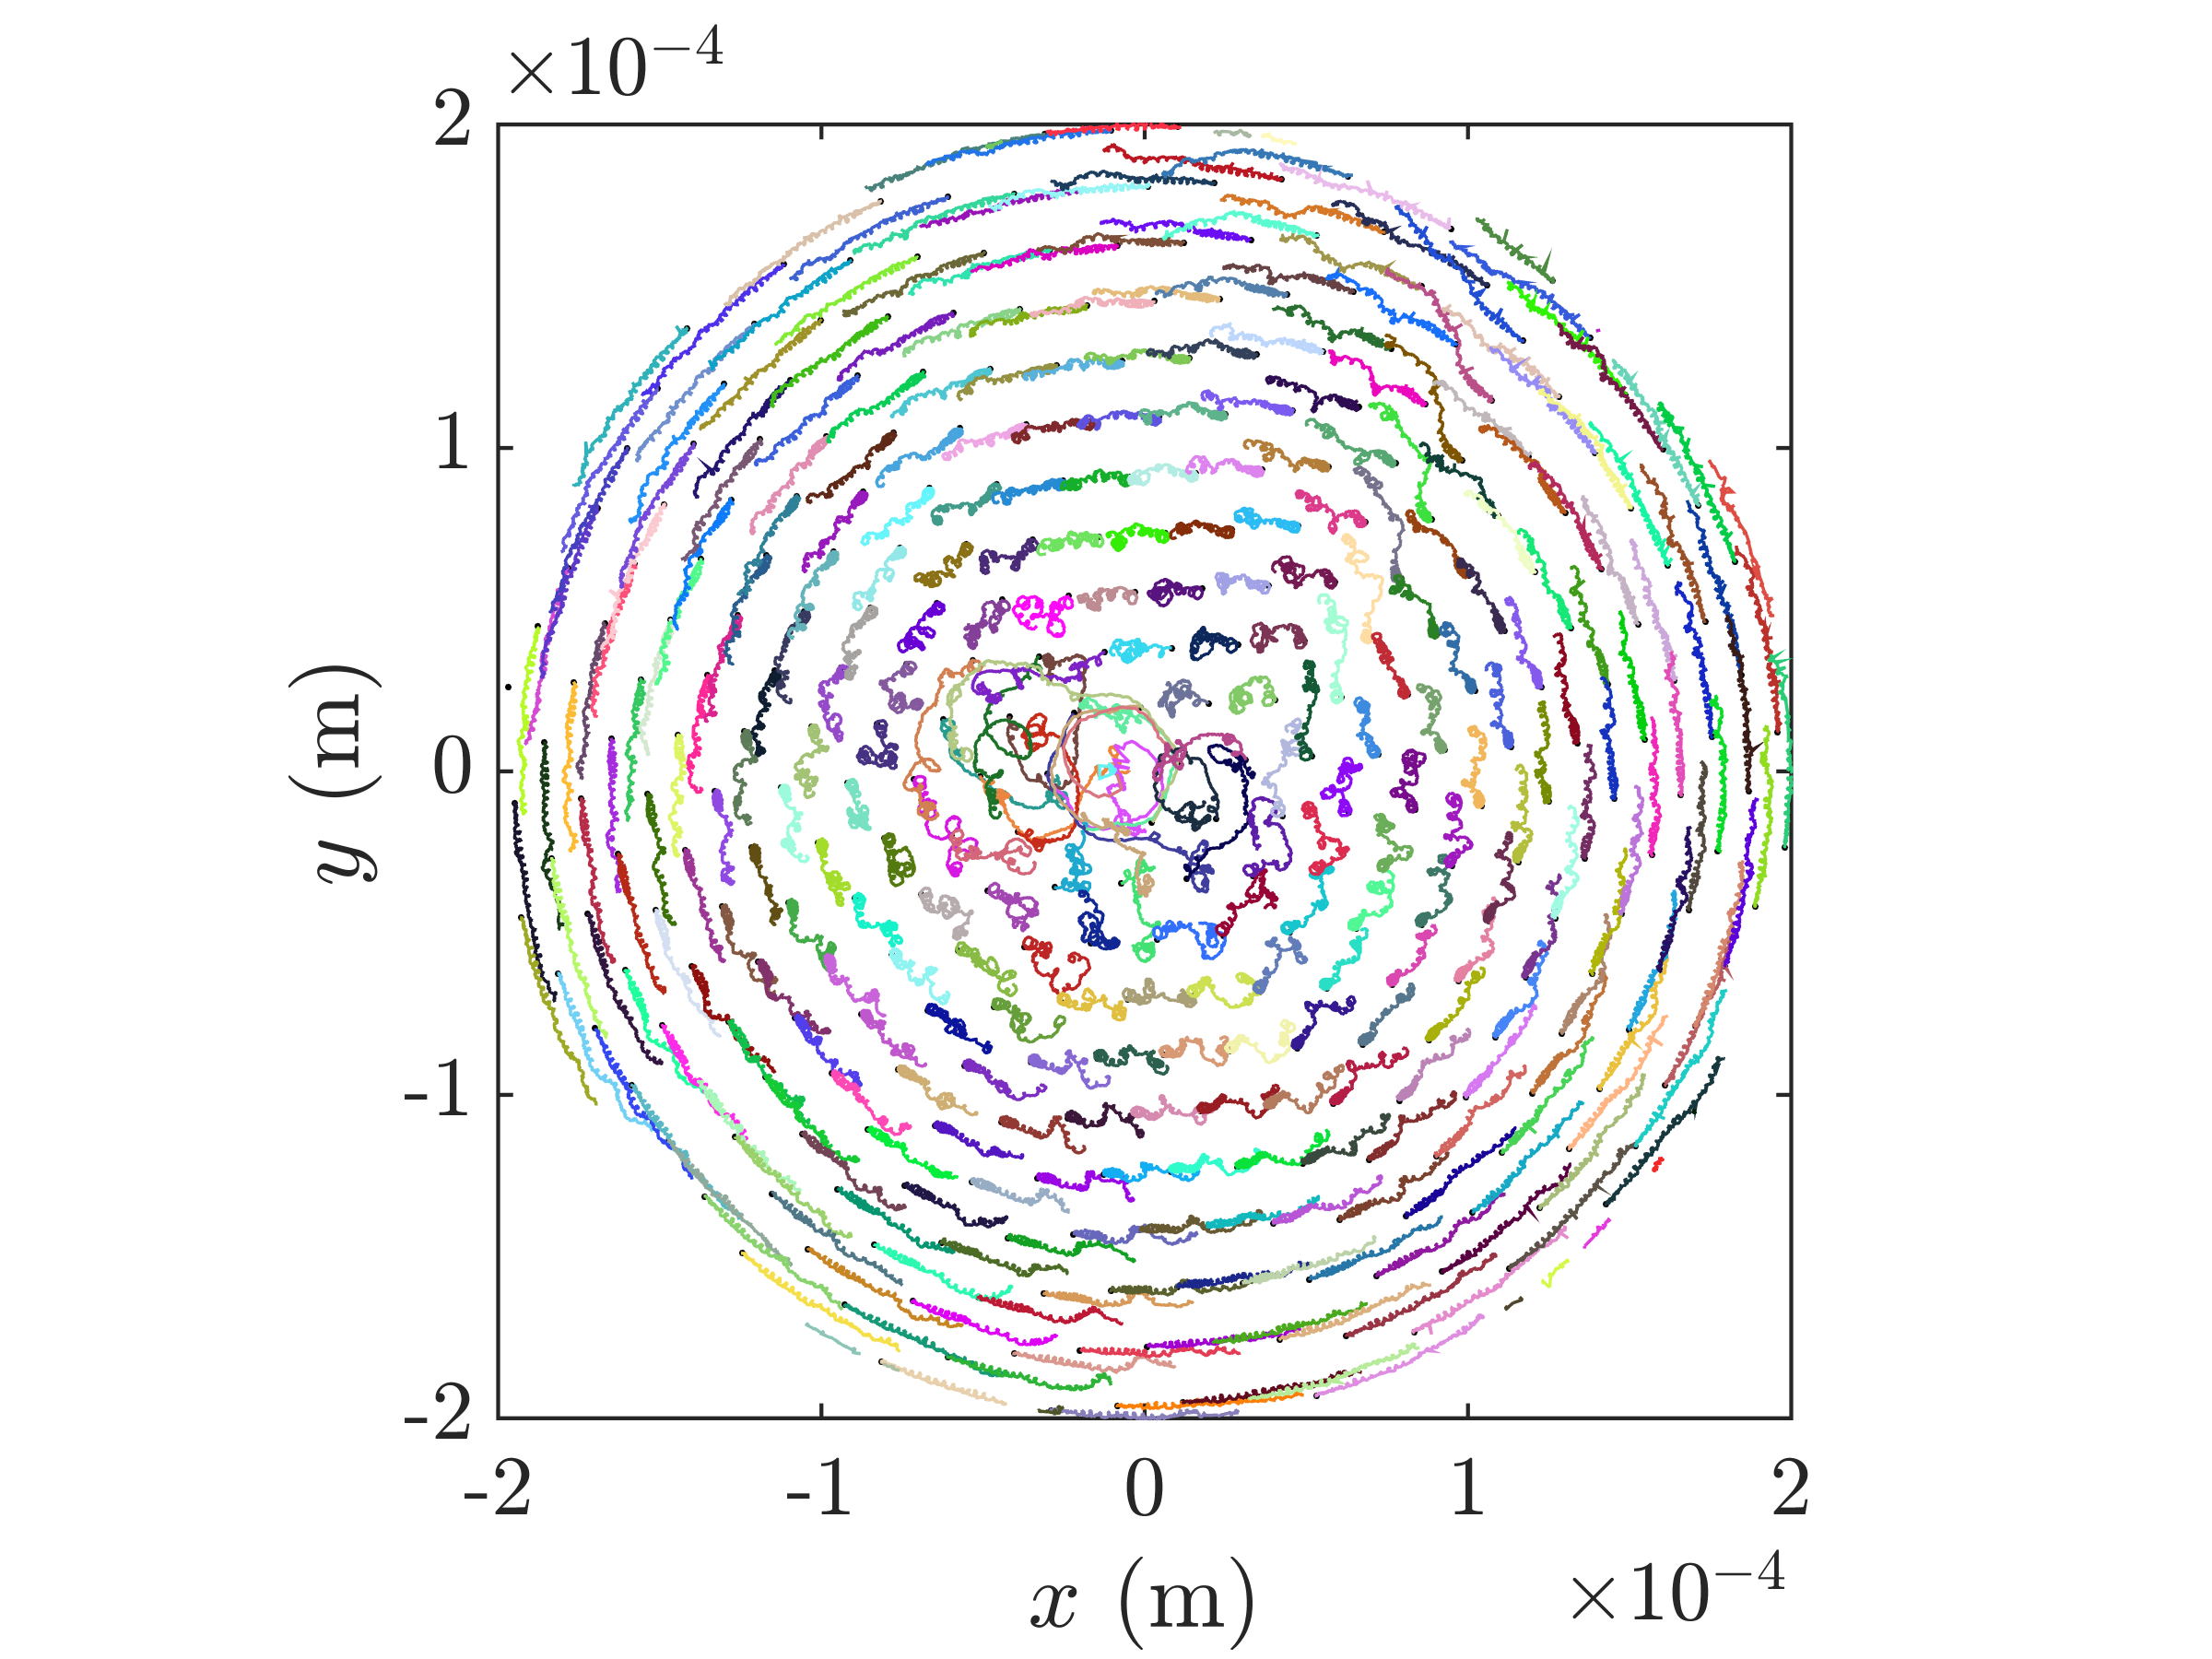
\includegraphics[width=0.55\textwidth, trim=0mm 0 0 0]{ch6_phasegineer/imgs/g2d/varr_161/Trajectory}
    \caption{The trajectories of the vortices over 10 s following a removal at the center shows a clear vacancy that remains into long times. The trajectories show almost perfect solid-body rotation of the lattice, with the only notable deviations resulting from the vortices adjacent to the vacancy.}
    \label{fig:trajplot}
\end{figure}

We remove a vortex from the centre of the vortex lattice, with a trajectory plot of the lattice following this removal over 10 s of time evolution given by Fig.~\ref{fig:trajplot}. The center of the lattice maintains a long-lived vacancy (order of seconds), with the adjacent vortices rotating faster than the lattice due to the loss of local velocity field. The stability of the nearest neighbour honeycomb-like structure is long lived, before eventually decaying akin to that described by \cite{Vtx:Leipold_jsm_2016}, creating a locally disordered region. This stable vacancy was observed irrespective of initial vortex choice provided it is within the region of constant areal density, though less stable than central placement. The overall vortex lattice remains well structured after a removal, as evidenced by examining the orientational correlation function given by Fig.~\ref{fig:g6}. It is interesting to note that the long-ranged behaviour following a removal has a higher correlation than without.

\begin{figure} \centering
    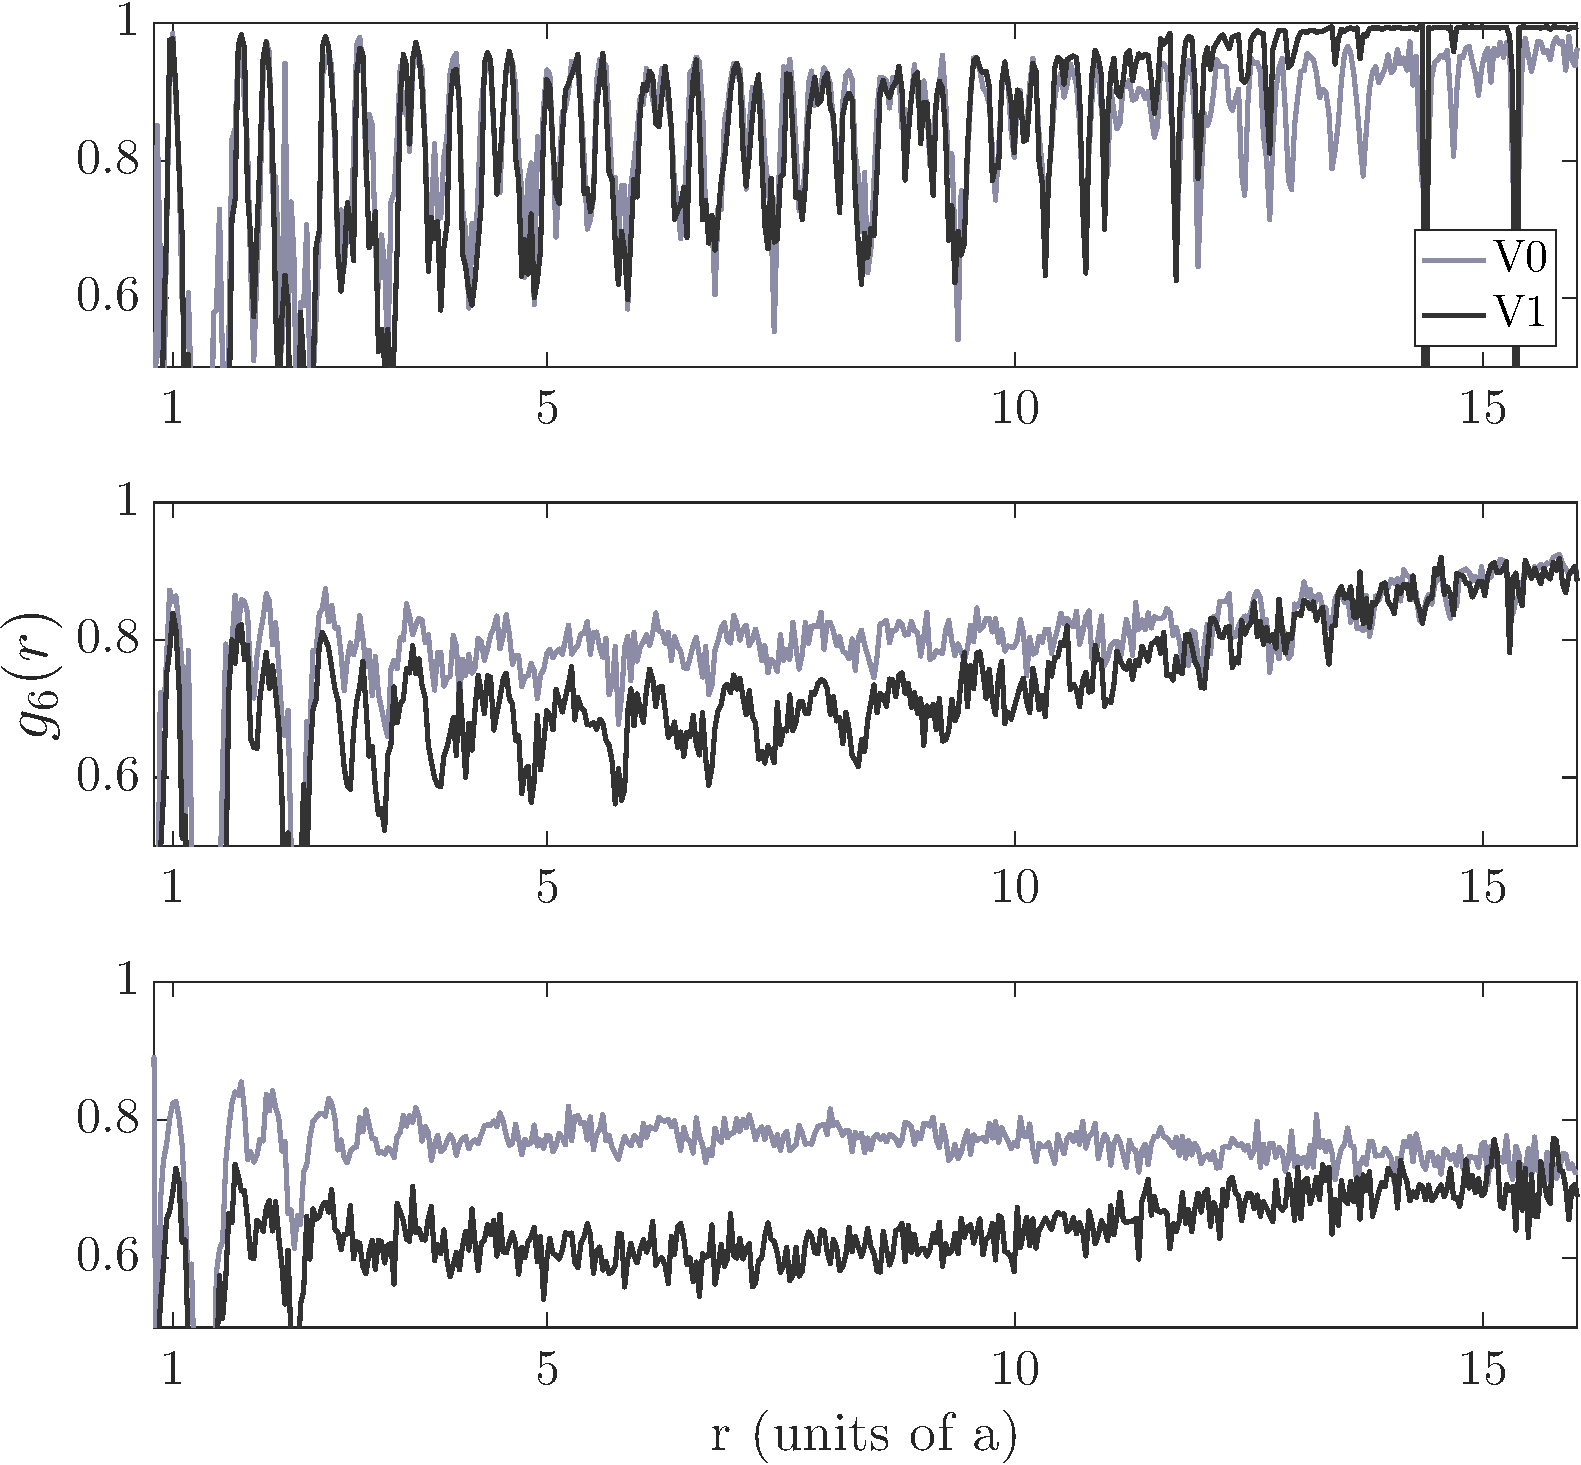
\includegraphics[width=0.55\textwidth]{ch6_phasegineer/imgs/NEWPICS/g6_varr0_varr161}
    \caption{The orientational correlation function for the unperturbed (V0) and central vortex removed (V1) are given for $t={1,4,10}$ s (t,m,b).}\label{fig:g6}
\end{figure}

The Delaunay triangulation of the lattice upon removing a single vortex is given in Fig.~\ref{fig:deltri_1vtx}. A pair of 5 and 7-fold defects act as a lattice dislocation, where two such pairs can be seen to remain localised and persist for long times following a vortex removal. Removing vortices at different positions in the lattice shows similar behaviour, with a localisation of the disordered region not far from the site of removal. Paired appearances of 5 and 7-fold connected edges indicate the presence of a dislocation, and we can measure the disorder of the lattice by counting the presence of these such defects. While generally not all 5 and 7-fold defects are paired due to the presence of $n$-fold connected vortices, coincidental appearance of these is good indication of a lattice dislocation.

\begin{figure} \centering
    \includegraphics[width=0.55\textwidth]{./ch6_phasegineer/imgs/NEWPICS/Delaunay_varr161.pdf}
    \caption{Delaunay triangulation of vortex lattice after removing 1 vortex, viewed at $t=\{0.01,0.8,2,10\}$ s. A pair of 5-7 dislocations persists in the lattice into long times.}\label{fig:deltri_1vtx}
\end{figure}

As a perfect vortex imprint may be challenging experimentally, as discussed earlier, we examine the situation where an imprint is not directly centred on a lattice vortex. For an Abrikosov vortex lattice in a rapidly rotating condensate, the core size becomes comparable to the distance between cores, allowing a core to be hit much more easily. Fig.~\ref{fig:lattice_misalign} gives a time-averaged examination of the number of lattice defects following an imprint relative to a vortex and lattice vector. The resulting lattice disorder is almost always comparable in the long time limit for perfect and imperfect alignment, with the number of defects observed to be on average between 1 and 4.  We can see that within the vortex core we have on average between 1 and 2 defects created for both 5- (a) and 7-fold (b) connected vortices. At the cusp of the core, the imprint tends to create upwards of 3 to 4, which again tends back to the average of 2 beyond this region. The previously discussed issue with the imperfect alignment thus is no longer problematic as in the low vortex number scenario. We will concentrate on the perfect imprint in future discussions.

\begin{figure} \centering
    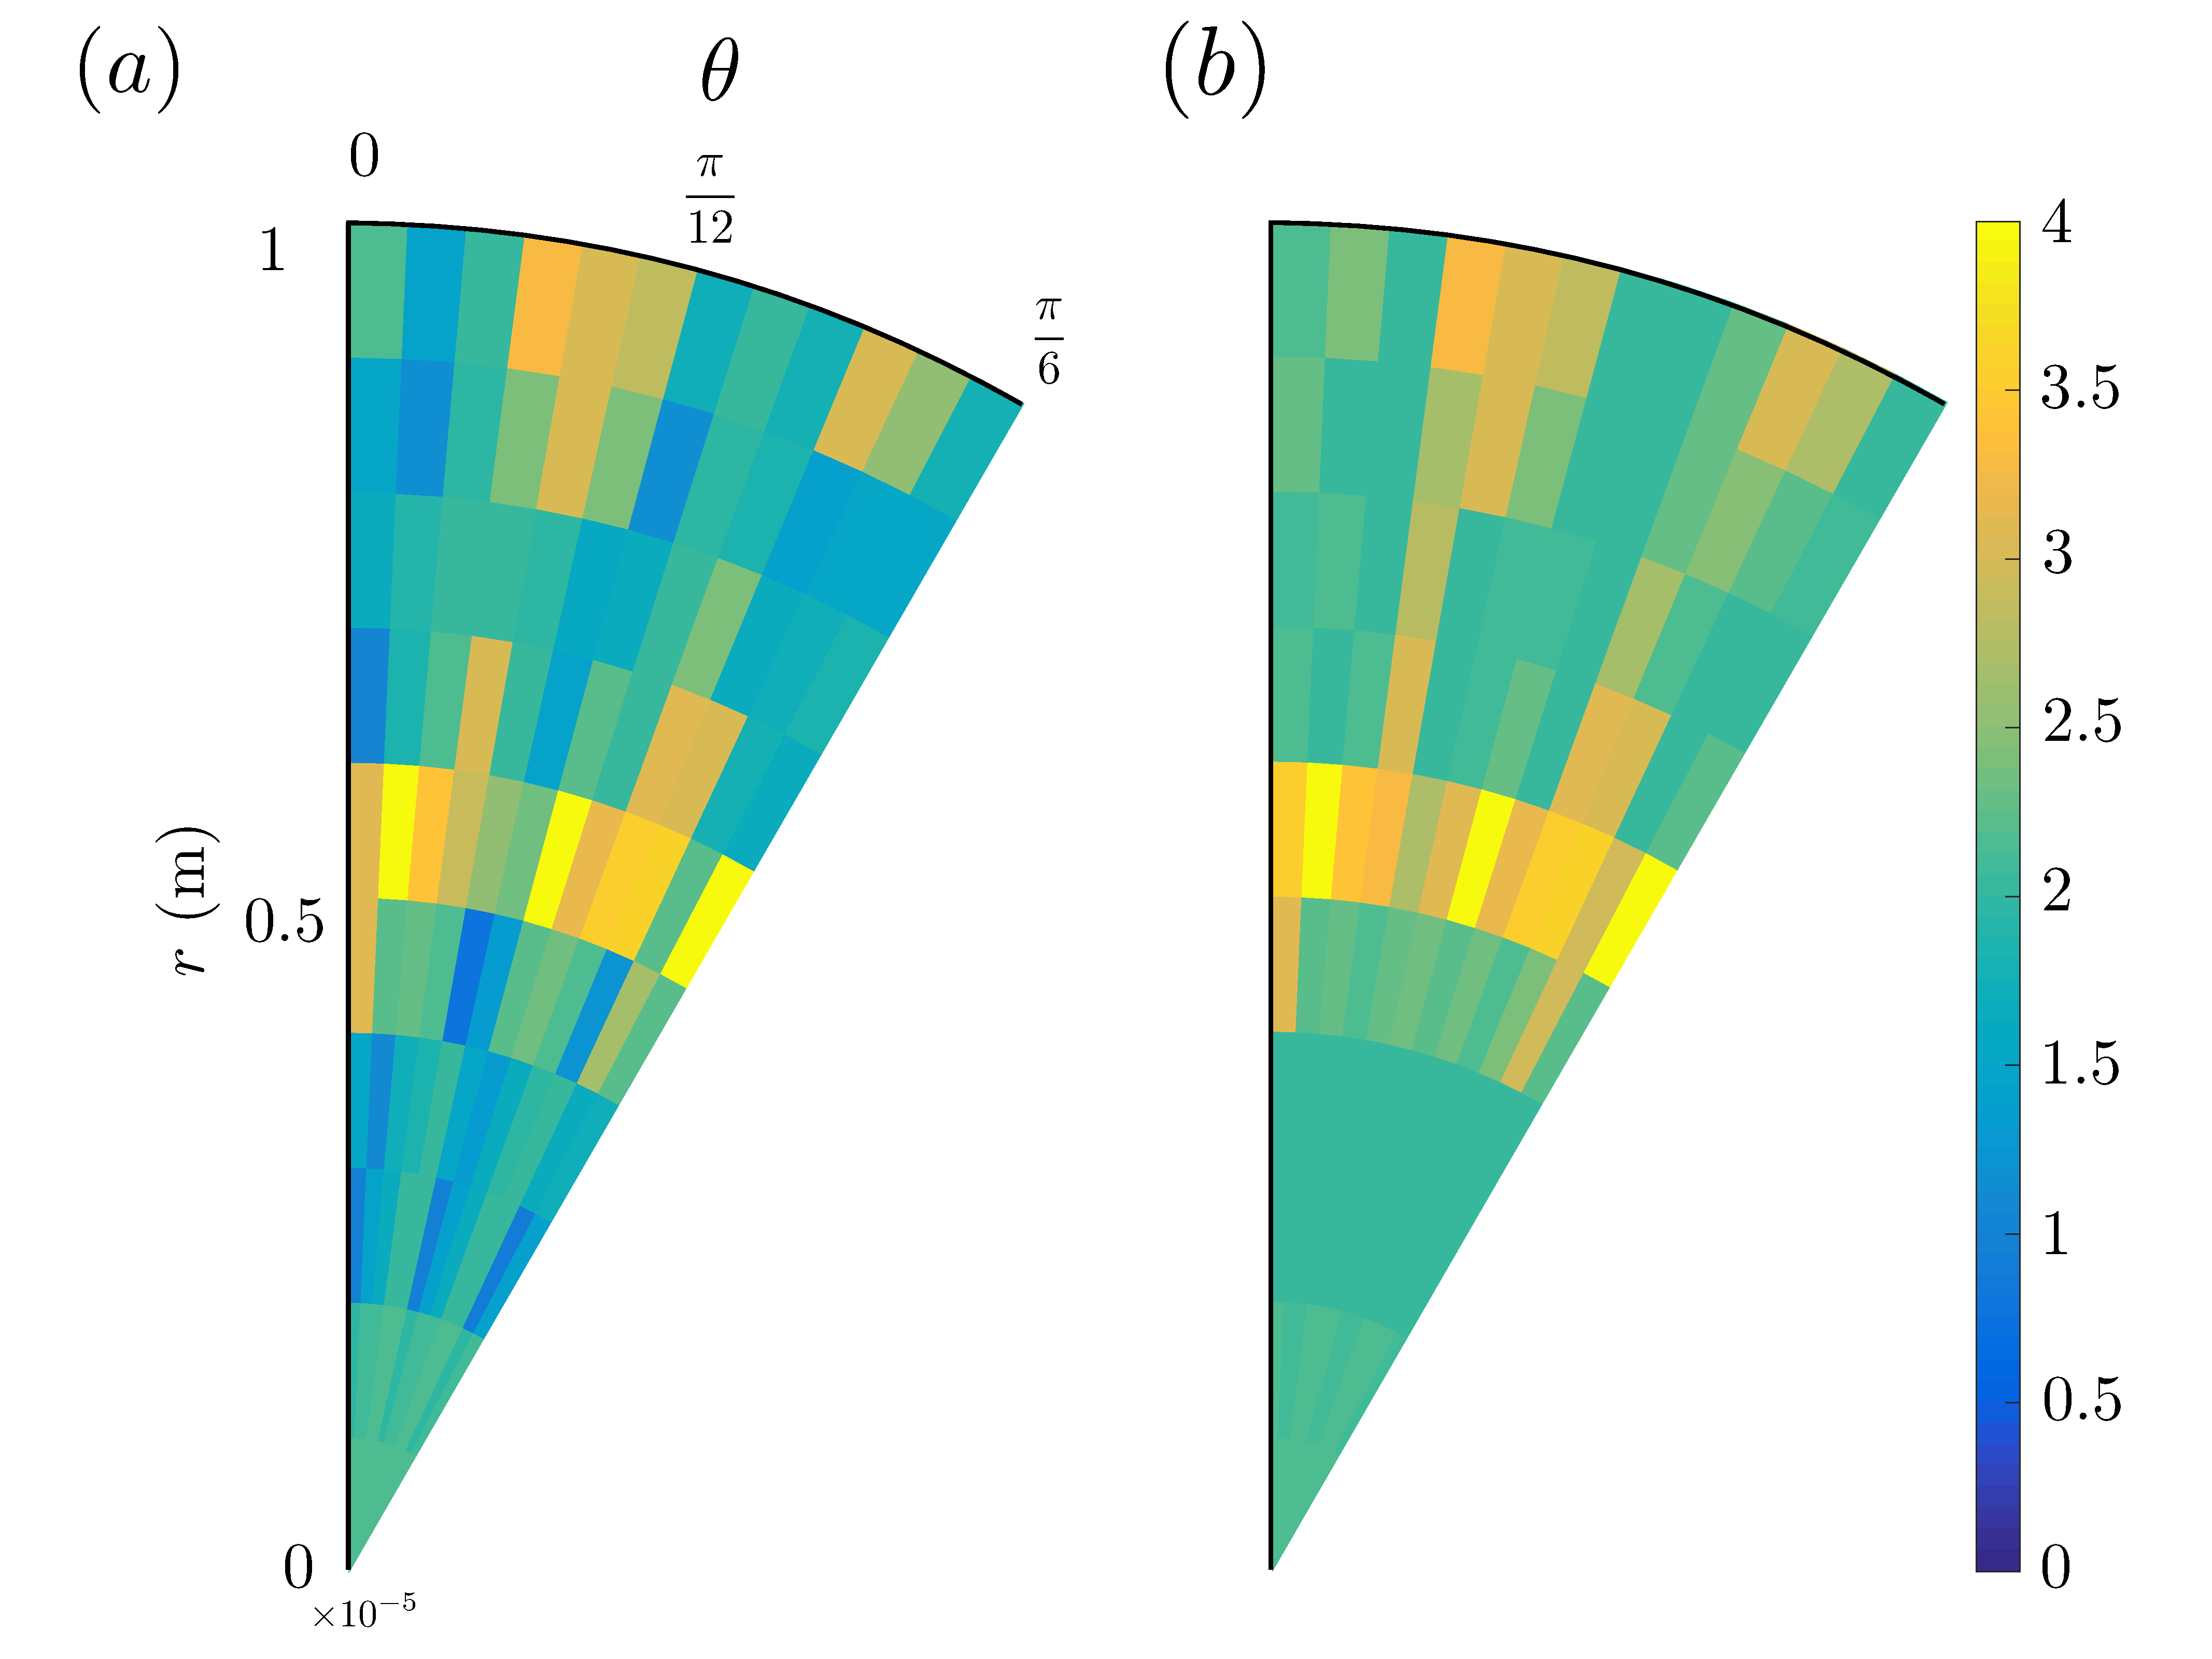
\includegraphics[width=0.55\textwidth]{ch6_phasegineer/imgs/NEWPICS/arc_def57.pdf}
    \caption{The time-averaged number of defects appearing over a range of imprint positions relative to a central vortex from $t=1\rightarrow$10 s, allowing 1 s of settling time. Both 5-fold (a) and 7-fold (b) defects are shown. A high coincidence is observed between their appearance, where a paired 5-7 defect indicates a lattice dislocation. Due to the presence of 4 and 8-fold defects additional counts can be observed when paired.} \label{fig:lattice_misalign}
\end{figure}

We can also examine the effect of removing more than one vortex from the lattice. Here we examine the case of removing two from a region away from the centre. Fig.~\ref{fig:traj_2vtx_edge} gives the trajectory plot of this, where we can again observe the localised vacancy and resulting defects in the lattice over 10 s of time. We track the number of edges formed between vortices, and plot this over time for 5, 6 and 7 nearest neighbours respectively ($N_x$), and we can observe such appearances as indicated by Fig.~\ref{fig:vtx_rem2_edge}. One can see that the behaviour is very similar to a singular imprint at the condensate centre.

\begin{figure} \centering
    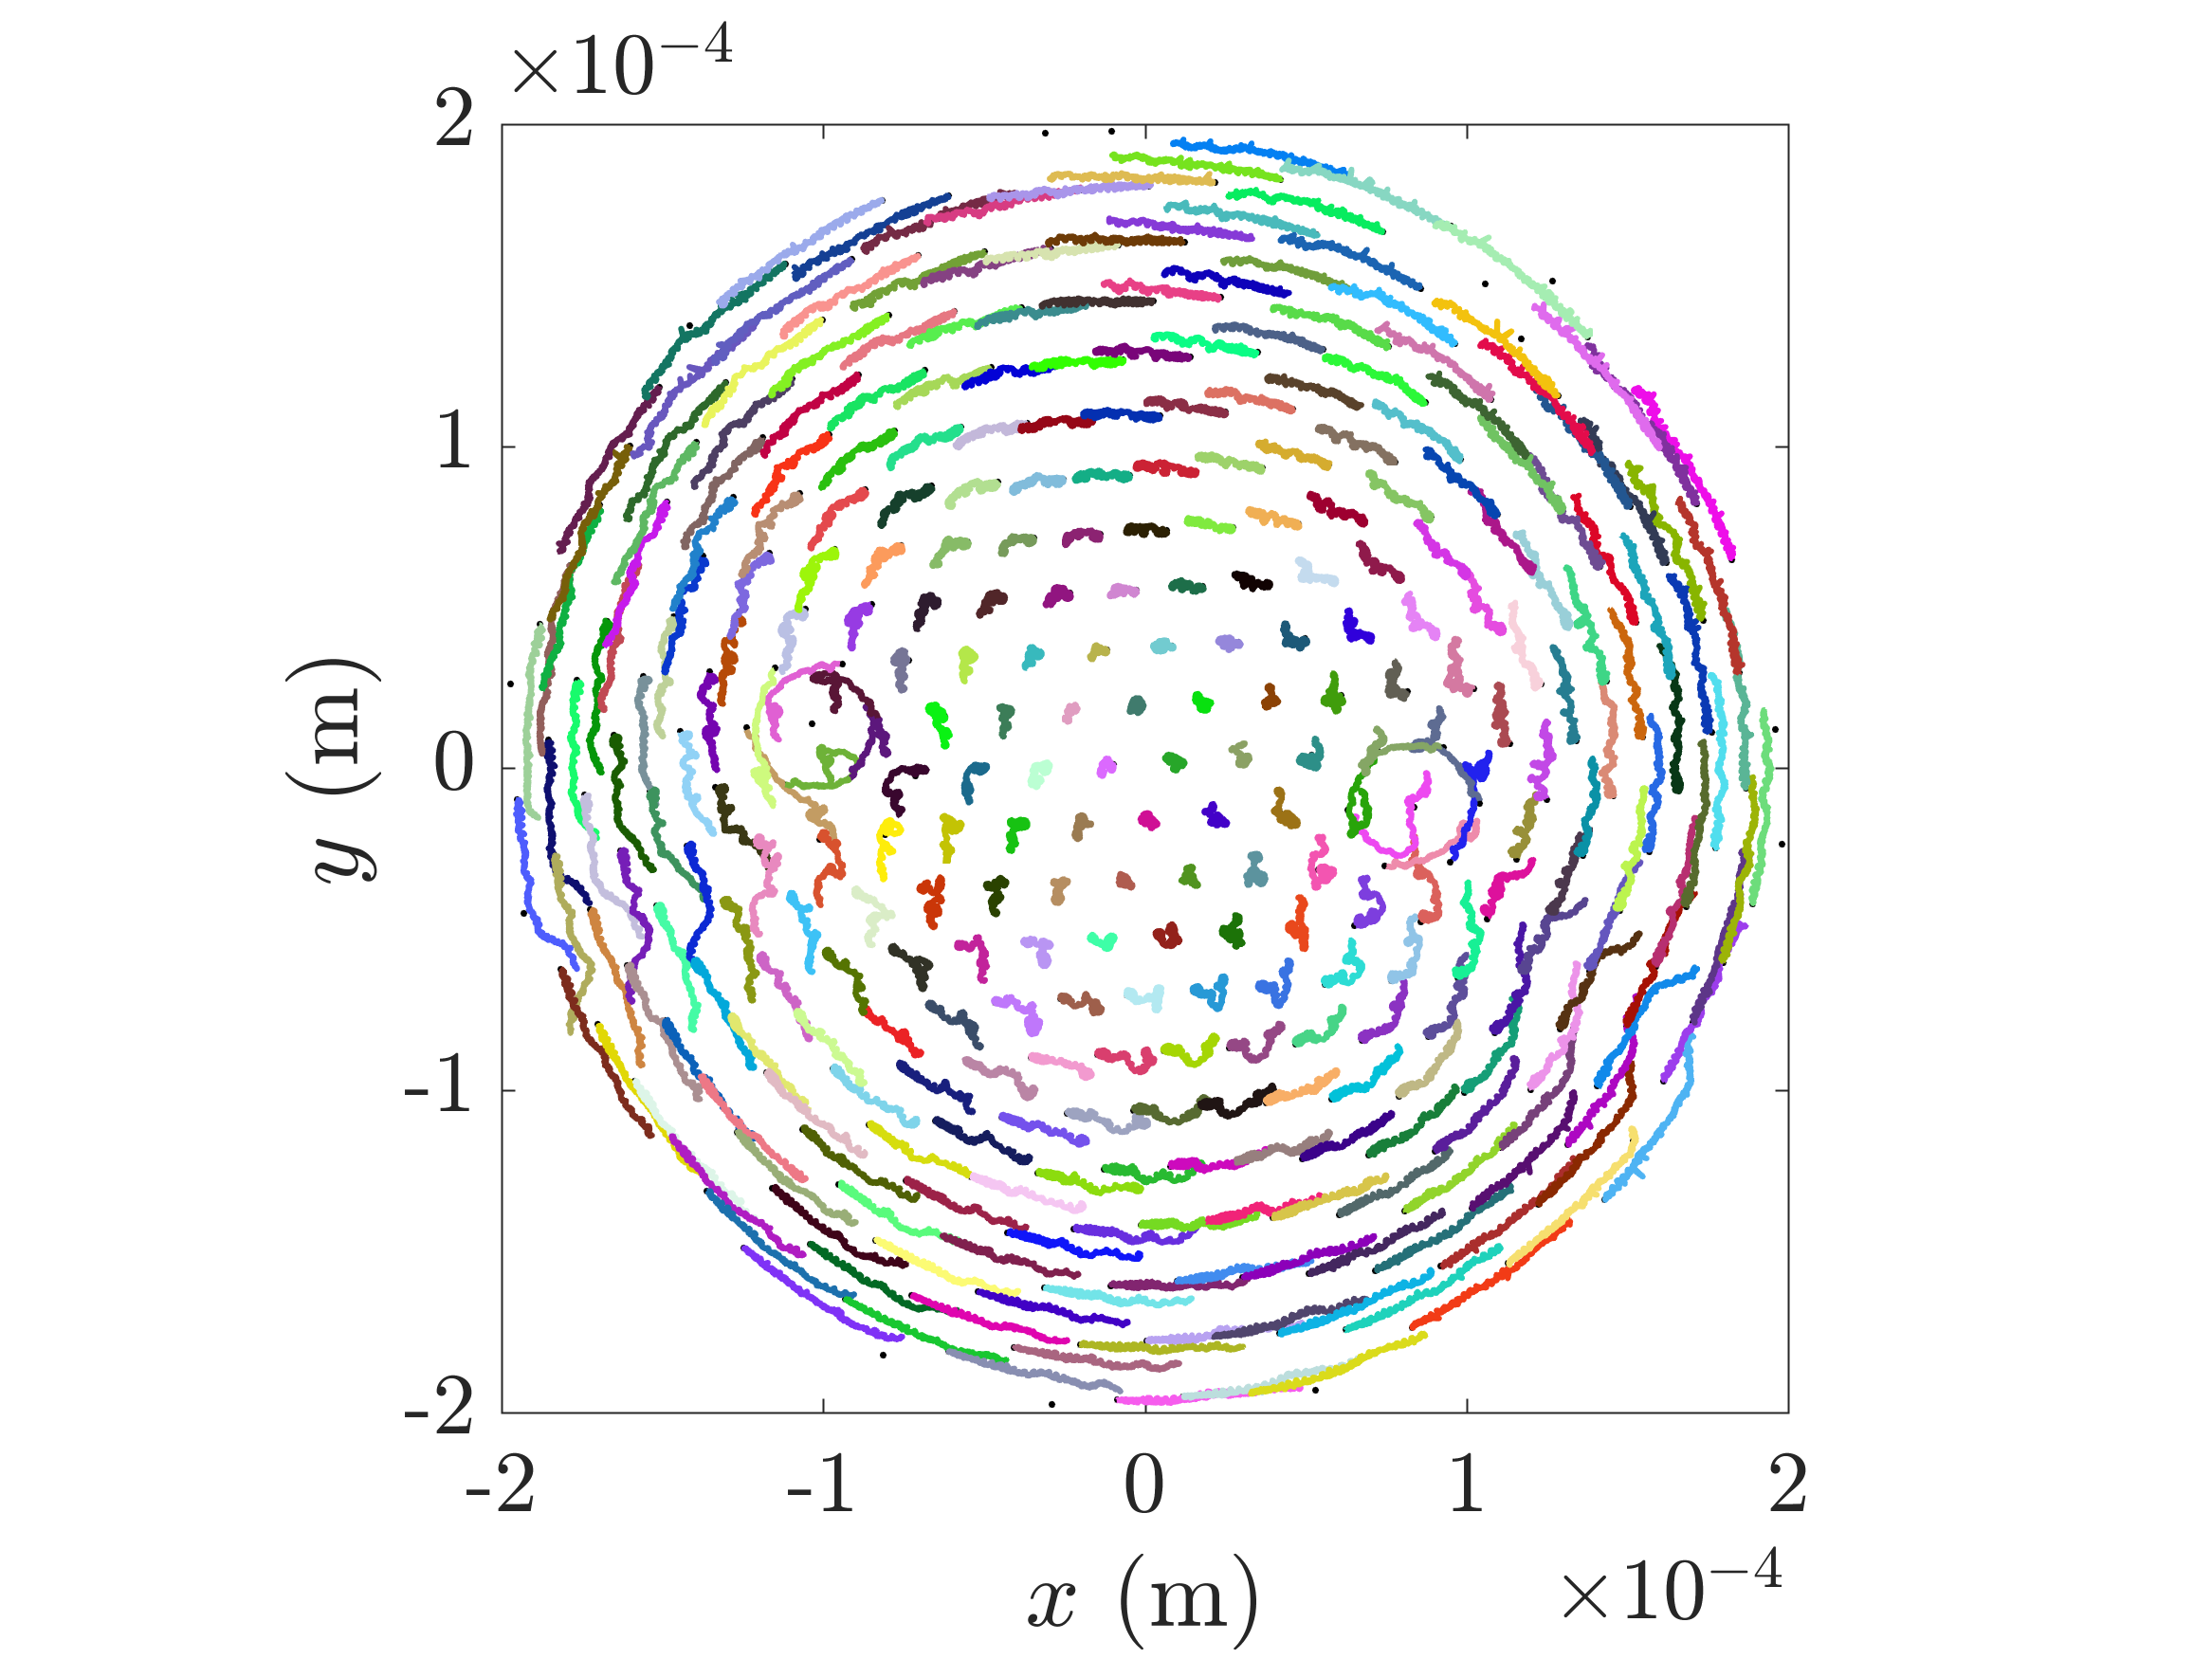
\includegraphics[width=0.55\textwidth,trim=0mm 0 0 0]{ch6_phasegineer/imgs/NEWPICS/Trajectory2edge.png}
    \caption{Vortex trajectories over 10 s upon removal of two vortices at either sides of the lattice show localised vacancies for long times. The lattice largely remains ordered as observed with removing the central vortex.}\label{fig:traj_2vtx_edge}
\end{figure}

\begin{figure} \centering
    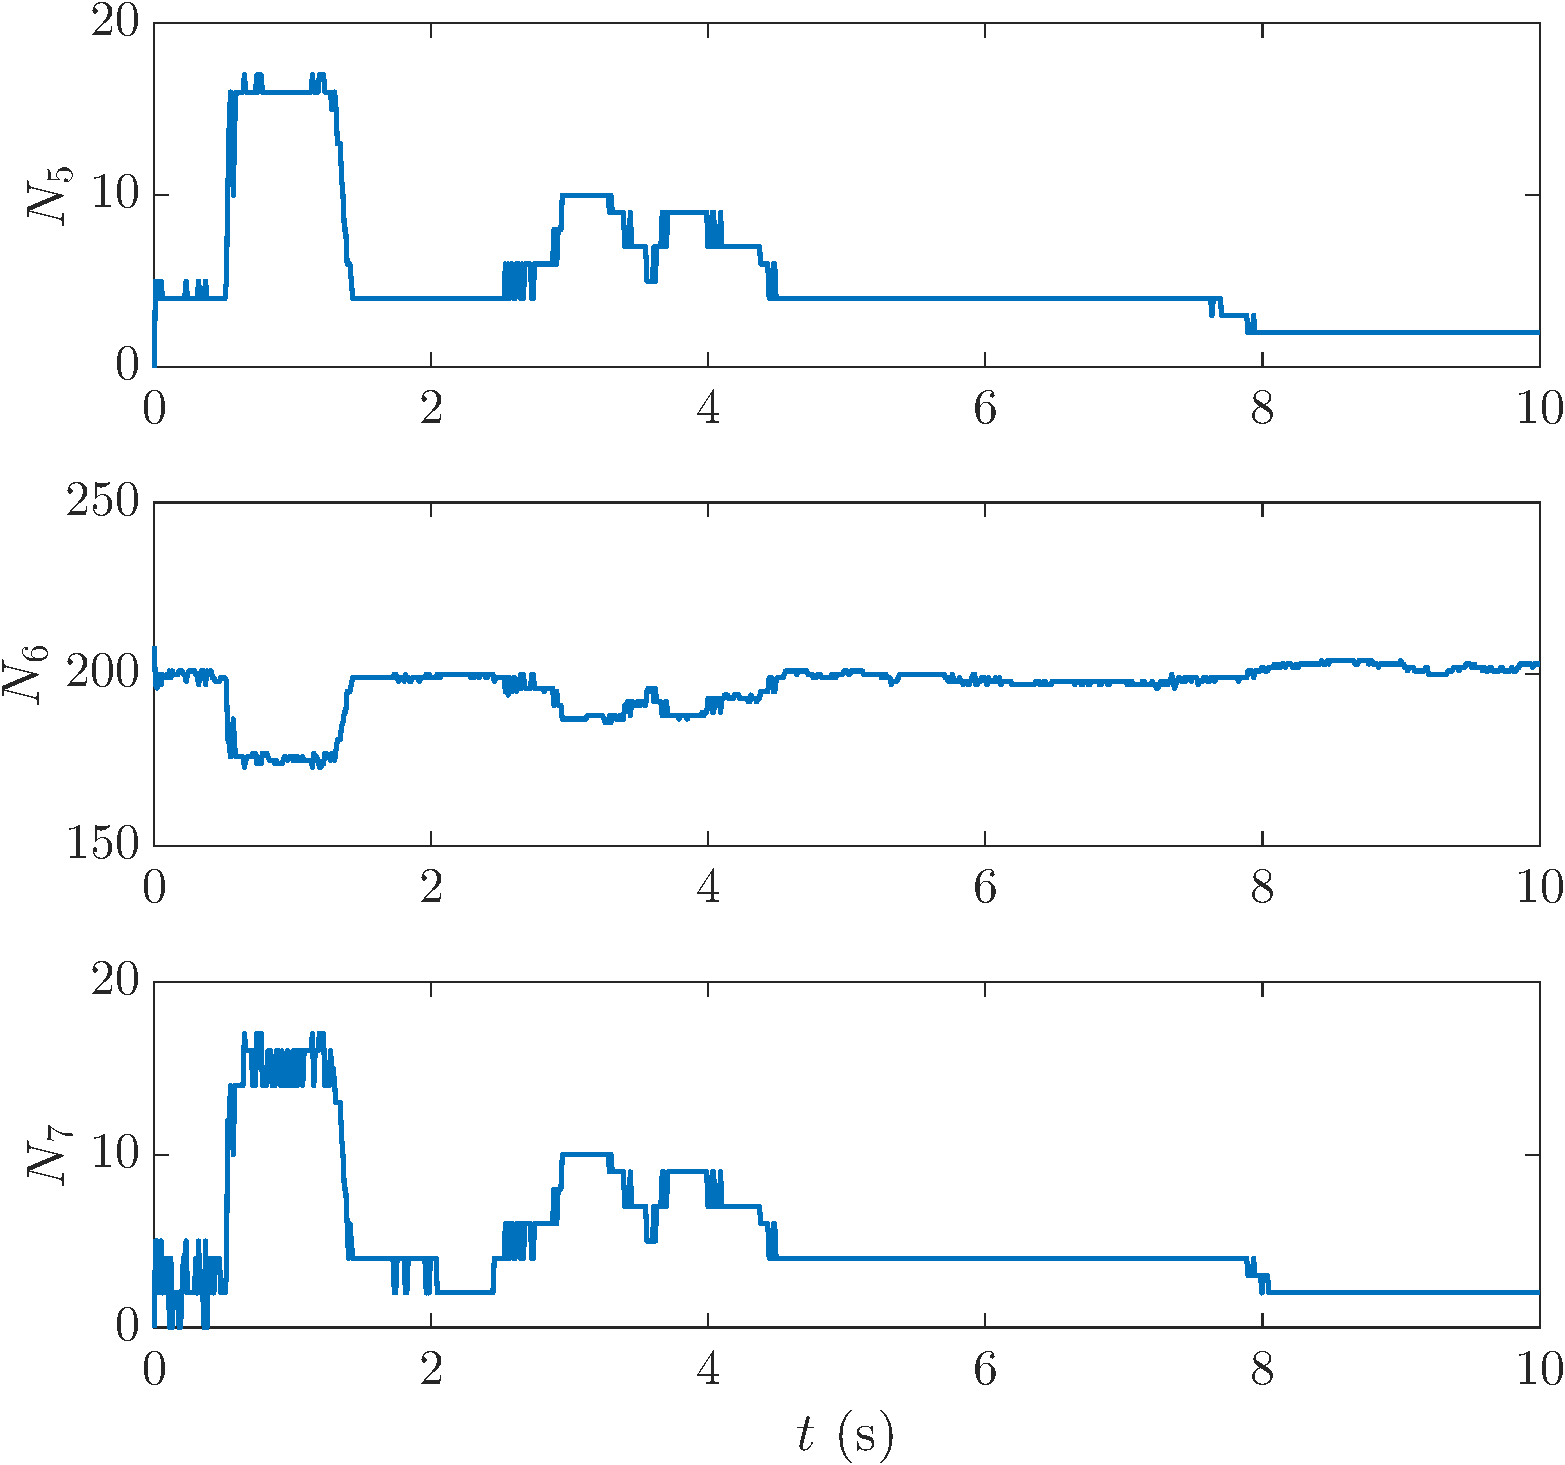
\includegraphics[width=0.55\textwidth]{ch6_phasegineer/imgs/NEWPICS/2edge_Defect57_t}
    \caption{The defect count taken from a Delaunay triangulation of the vortex lattice following the removal of 2 vortices on opposite sides. After a brief settling time, the lattice attains an almost constant defect count with between 2 and 4 vortices, depending upon time.}\label{fig:remove7_defect}
    \label{fig:vtx_rem2_edge}
\end{figure}

%%%%%%%%%%%%%%%%%%%%%%%%%%%%%%%%%%%%%%%%%%%%%%%%%%%%%%%%%%%%%%%%%%%%%%%%%%%%%%%%%%%%%%%%%%%%%%%%%%%%%%%%%%%%%%%%%%%%%%%%%%%%%%%%%%%%%%%%%%%%%
%\subsection{Vortex dynamics and lattice defects}\label{sec:numerics}
%%%%%%%%%%%%%%%%%%%%%%%%%%%%%%%%%%%%%%%%%%%%%%%%%%%%%%%%%%%%%%%%%%%%%%%%%%%%%%%%%%%%%%%%%%%%%%%%%%%%%%%%%%%%%%%%%%%%%%%%%%%%%%%%%%%%%%%%%%%%%

We can also use the phase imprinting as a means to create a varying degrees of disorder. By applying the appropriate $4\pi$ magnitude phase imprint we can replace a vortex with an antivortex at a required position. Given that the density depletion already exists, this simply flips the rotation of direction of the velocity field around the vortex. However, it is immediately obvious that such a situation is unstable, which can be observed by the onset of defects in Fig.~\ref{fig:varr161anti_defect}. One can observe an almost linear behaviour until approximately $t=1$ s, wherein the antivortex causes local disordering of the lattice, annihilates with a nearby vortex, and gives rise to the creation of a large number of 5-7 dislocations. Between $t=3$ and $t=4$ s we can observe the number of defects no longer growing, but instead fluctuate about a stable value.

\begin{figure} \centering
    \vspace{1cm}
    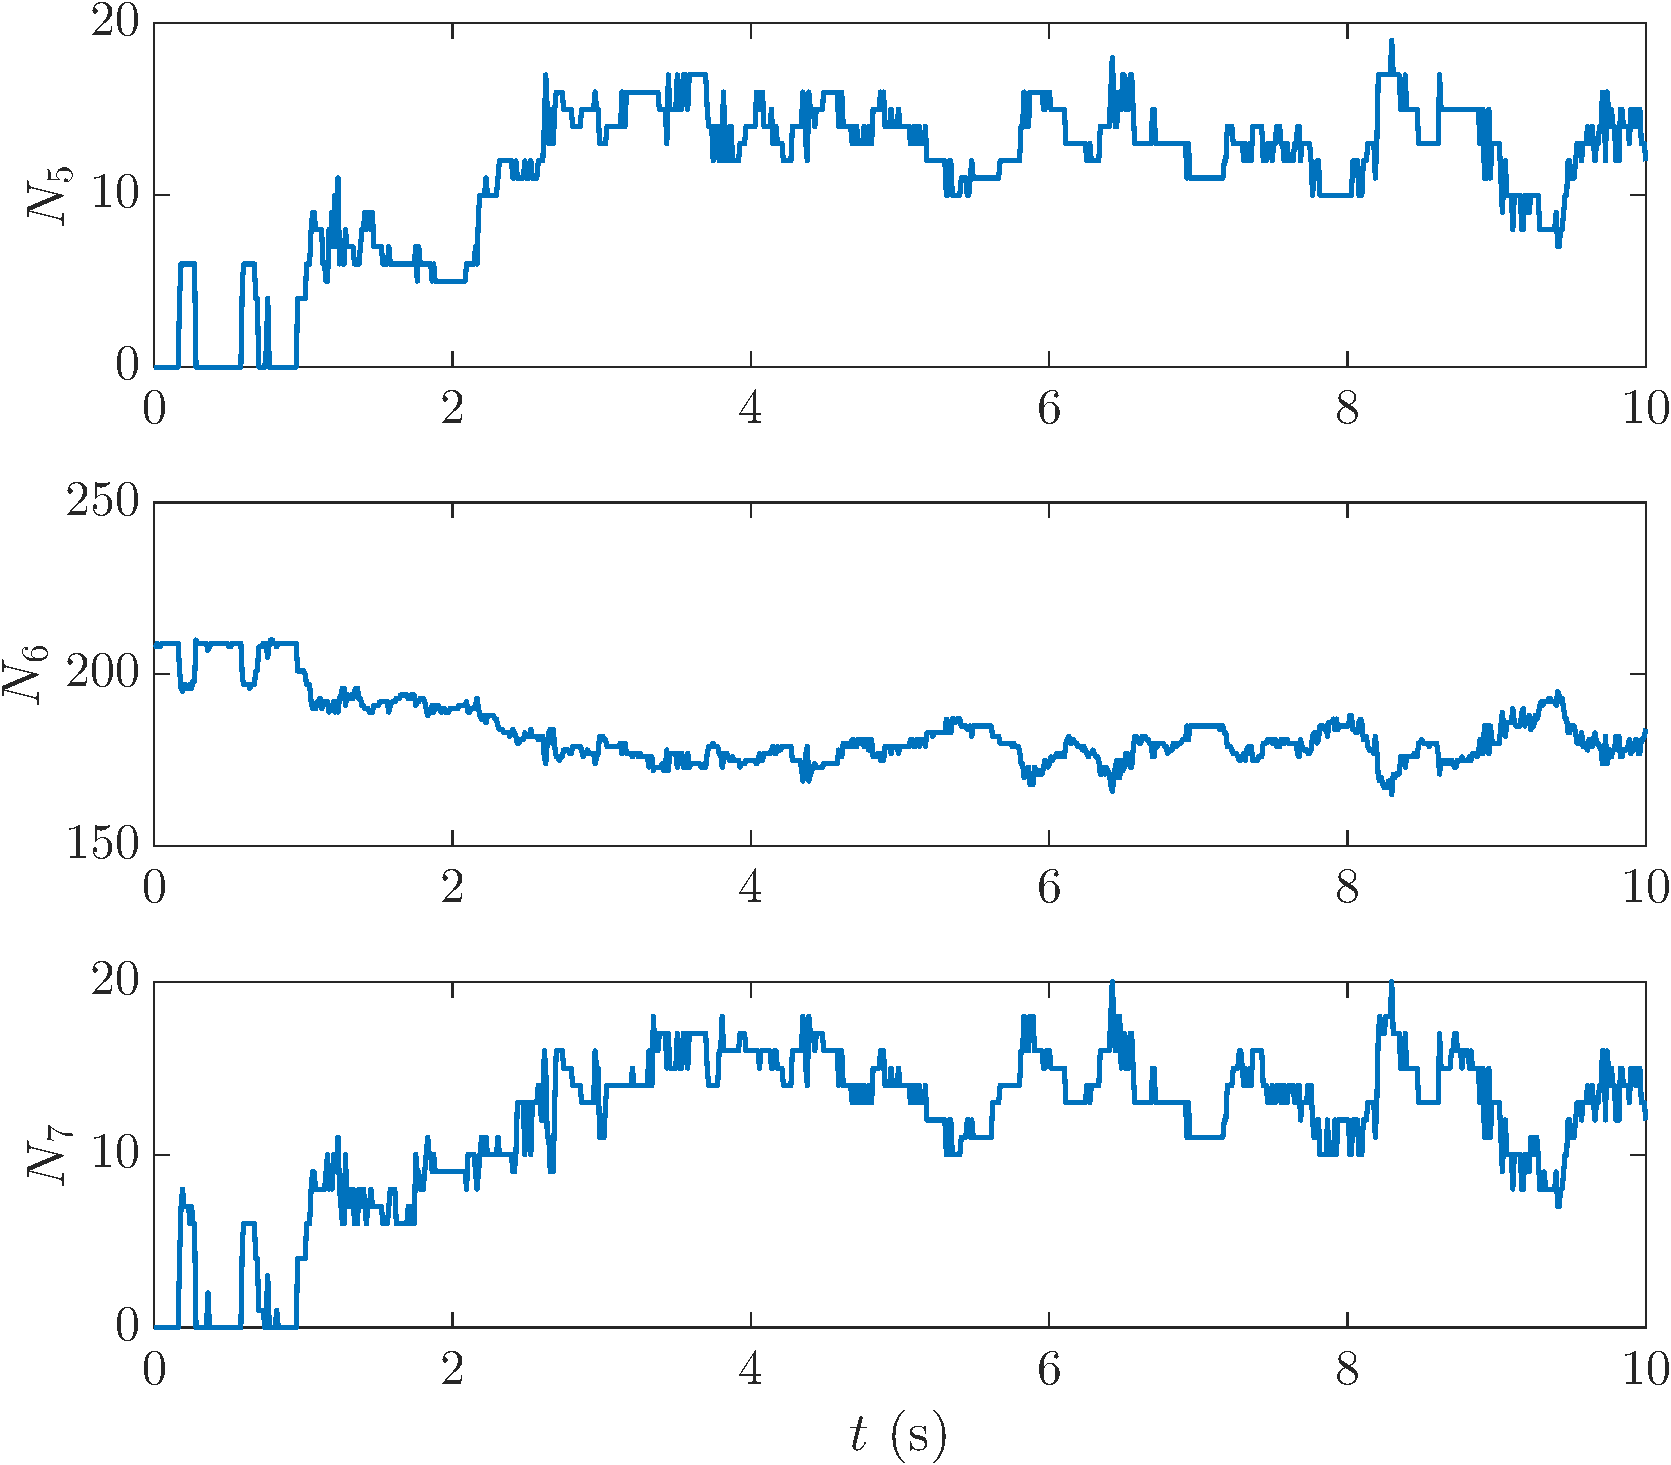
\includegraphics[width=0.55\textwidth]{ch6_phasegineer/imgs/NEWPICS/Defect57_varr161anti.pdf}
    \caption{The defect count taken from a Delaunay triangulation of the vortex lattice following an insertion of an antivortex. The number of defects increases largely as the local structure decays, and eventually gives rise to a constant-plus-fluctuations region of defect numbers.}\label{fig:varr161anti_defect}
\end{figure}

While we have shown that it is possible to create low and moderate numbers of long-lived 5-7 dislocations in an Abrikosov vortex lattice controllably, we can create a large amount of disorder in the lattice using these techniques also. We can choose to remove an entire 7 vortex triangular lattice cell from the condensate and observe the resulting effects on the remaining lattice. In this instance, the number of lattice defects rises considerably, and continues to rise until the simulation end, shown by Fig.~\ref{fig:remove7_defect}. In this case, the disordered regions occupy a large degree of the lattice, with the number of 6-fold connected vortices now dropping sharply.

\begin{figure} \centering
    %\vspace{1cm}
    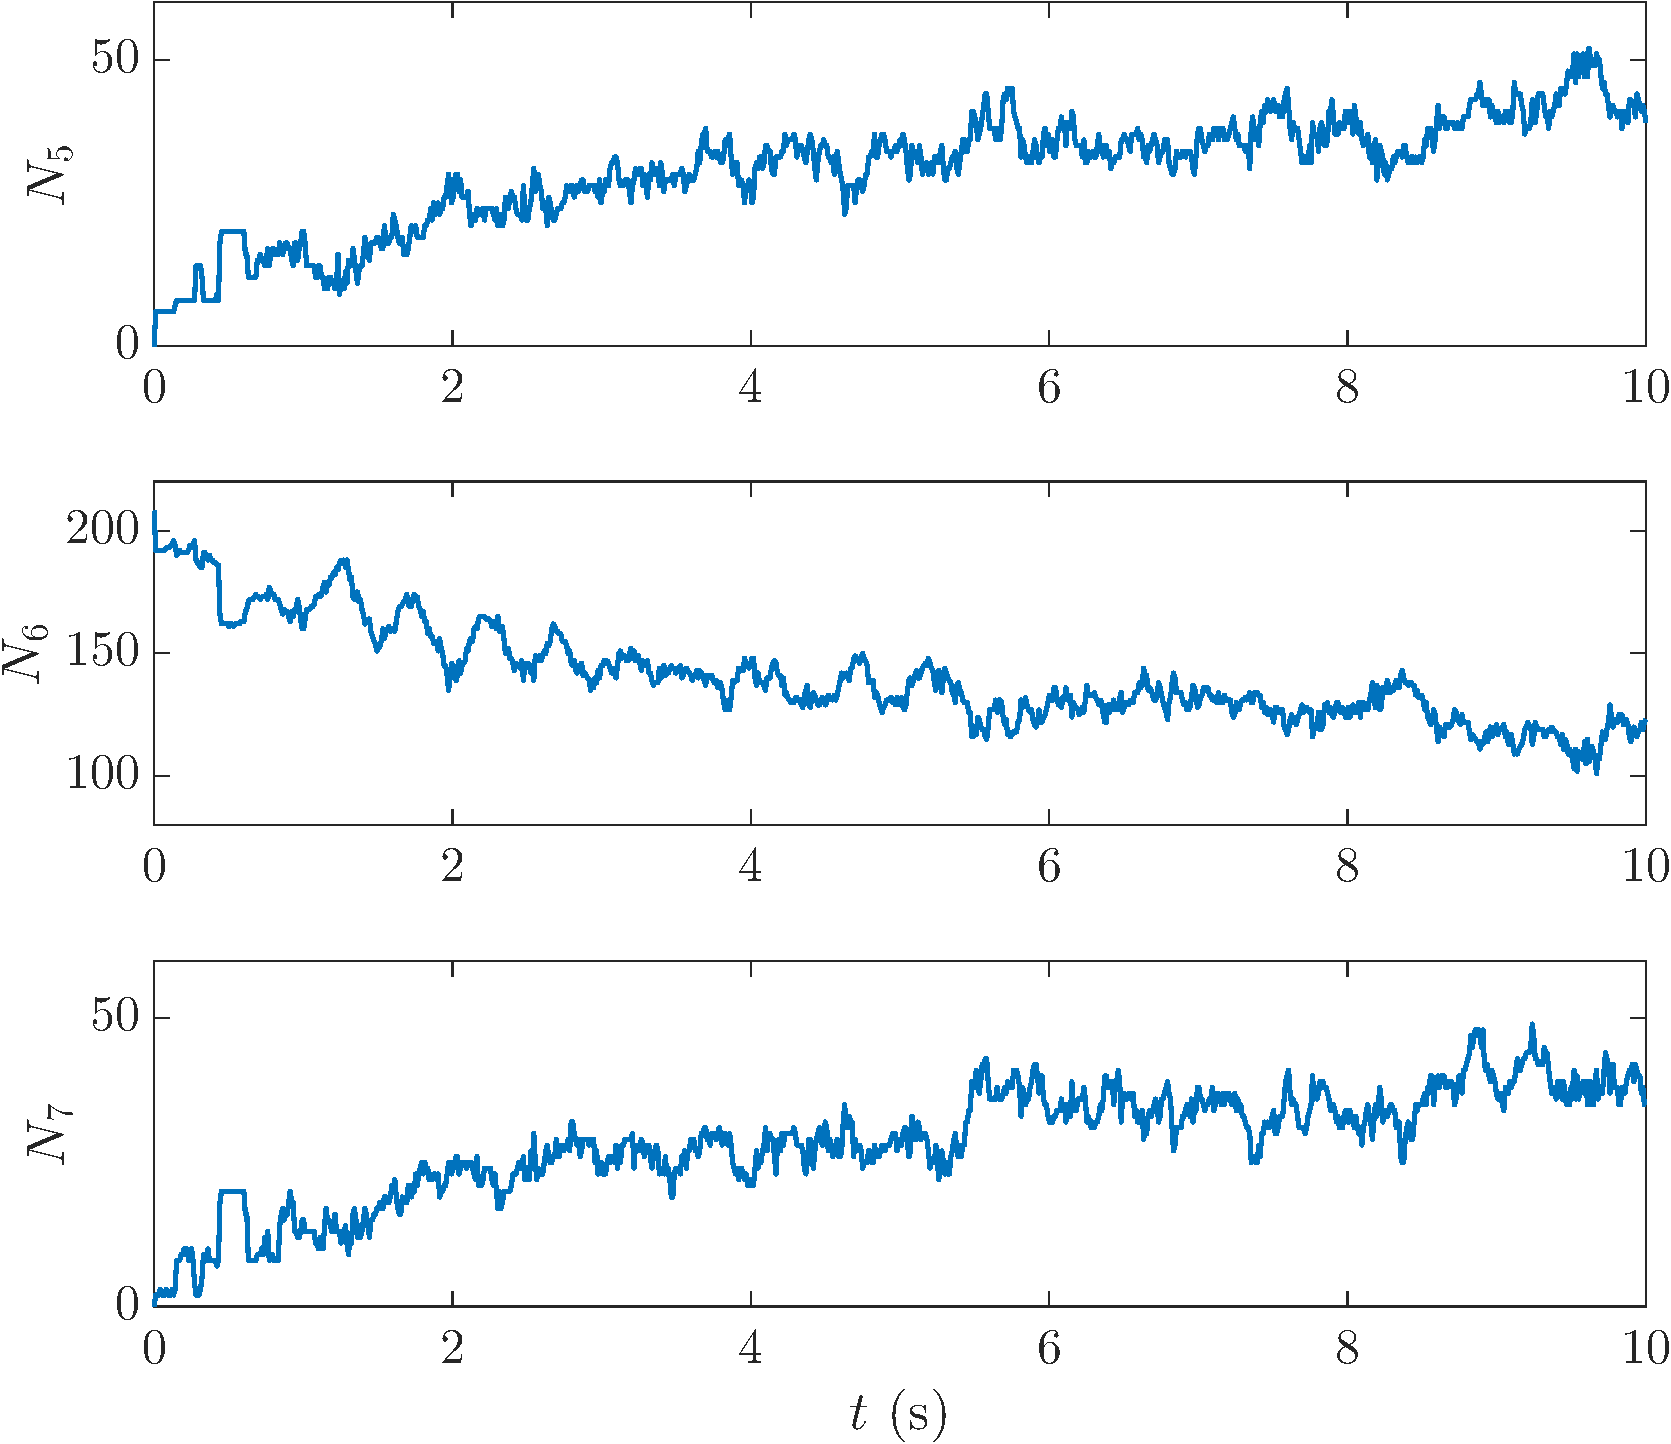
\includegraphics[width=0.55\textwidth]{ch6_phasegineer/imgs/NEWPICS/Defect57_nuclear.pdf}
    \caption{The defect count taken from a Delaunay triangulation of the vortex lattice following the removal of 7 vortices. Defects can be seen to rise as a function of time.}\label{fig:remove7_defect}
\end{figure}

Comparing the orientational correlation function for removing 2, creating an antivortex, and removing 7 vortices shows a clear distinction in the lattice order (see Fig.~\ref{fig:g6_2edge_anti_nuclear}). A removal of 2 vortices at opposite sides of the condensate yields high correlations across all times and length scales, indicating a well ordered lattice. For creating an antivortex in the lattice the correlations are lower across length scales in the long time limit, but tend to the same long-ranged value as the previous case. We can interpret this as the presence of ordering of the lattice outside the regions of localised defects. Lastly, comparing the removal of 7 vortices, we see a singificant drop in correlations at all length scales and across both times. We can interpret this as a global disordering of the vortex lattice, as indicated by the large number of defects indicated earlier.

\begin{figure} \centering
    %\vspace{1cm}
    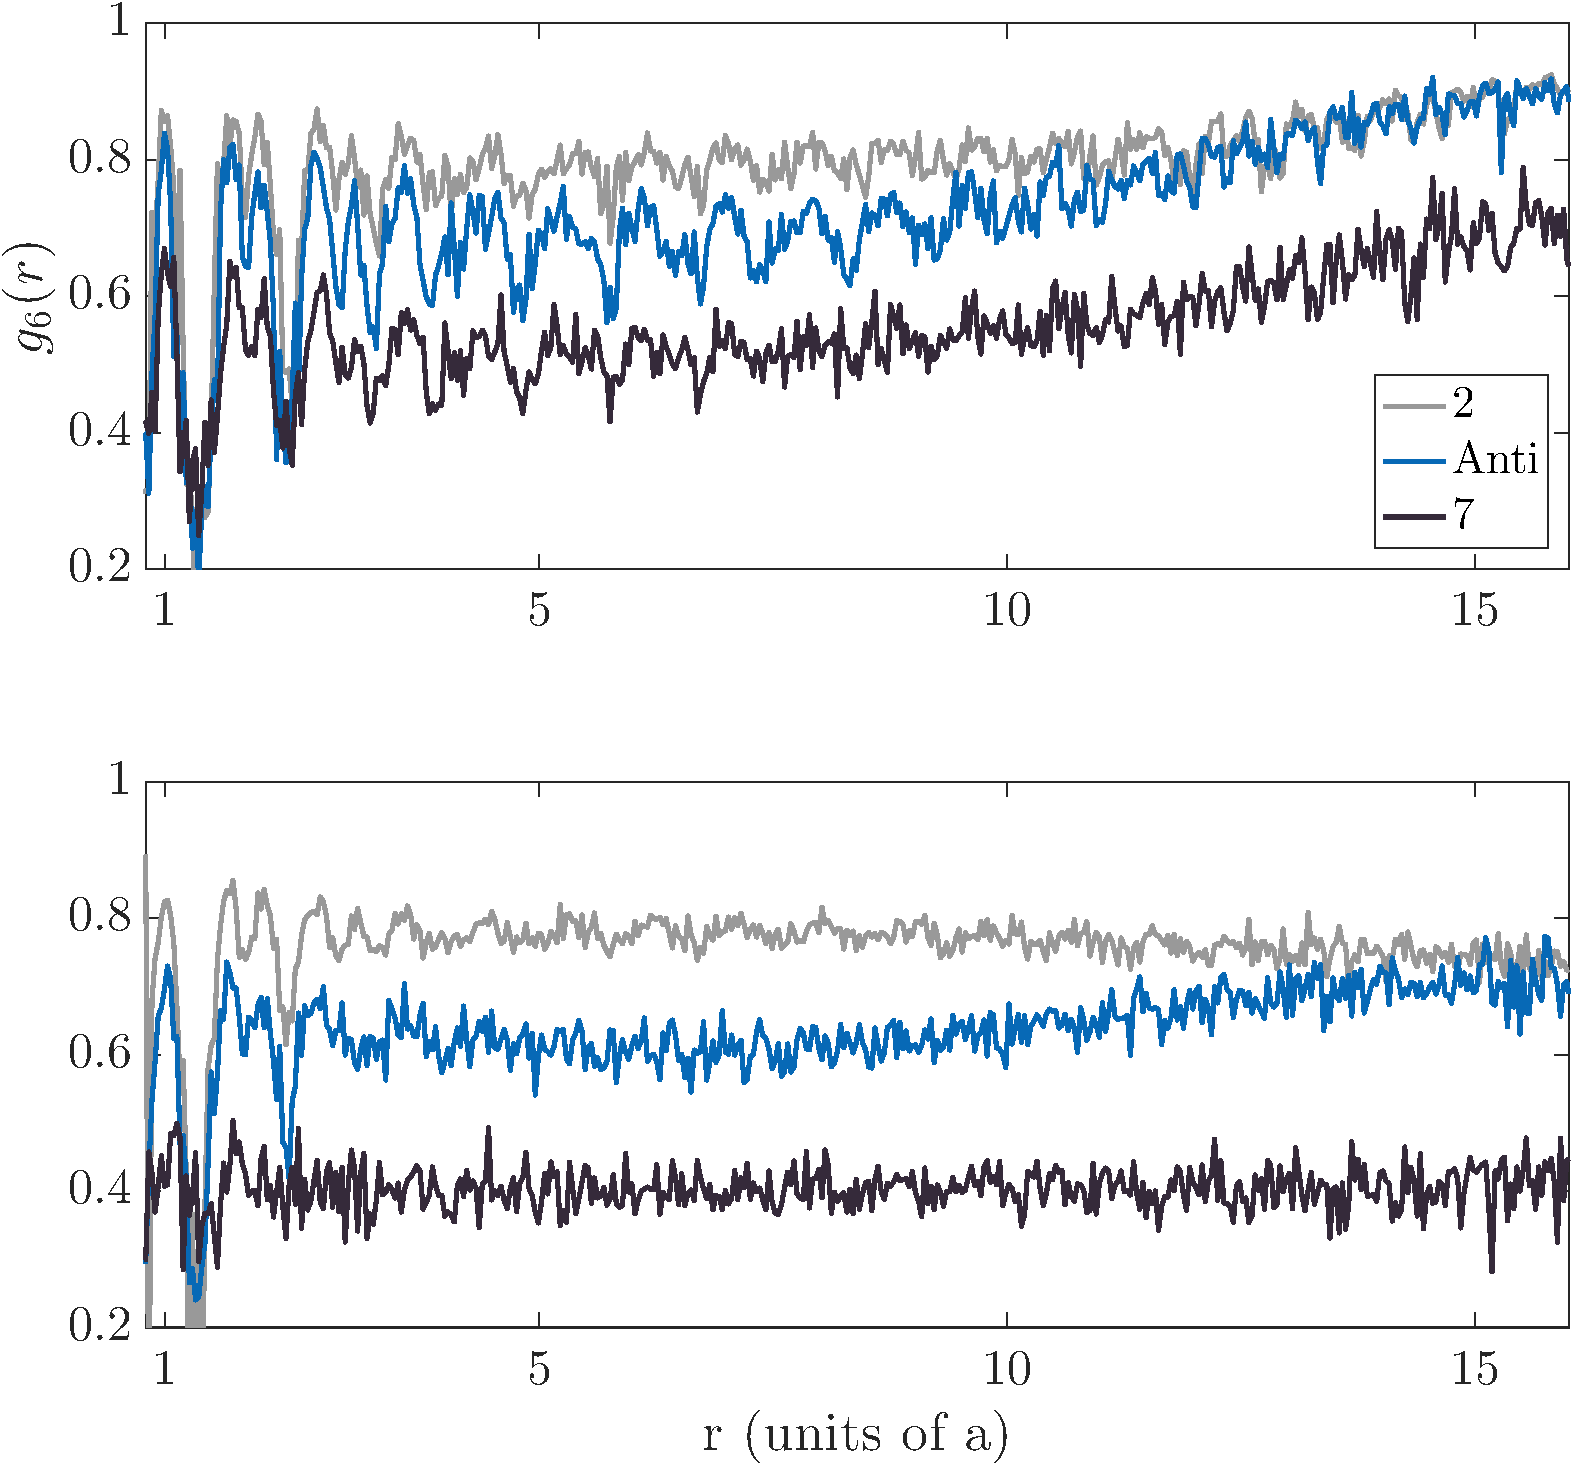
\includegraphics[width=0.55\textwidth]{ch6_phasegineer/imgs/NEWPICS/g6_2edge_anti_nuclear.pdf}
    \caption{The orientational correlation function is given for moderate ($t=4$ s, top) and long ($t=10$ s, bottom) times. Short range order is clearly distinct between all three cases, with long range comparable for both removing 2 non-central and creating an antivortex at moderate and long times. Removing 7 vortices significantly lowers correlations across all length scales, indicating a globally disordered lattice.}\label{fig:g6_2edge_anti_nuclear}
\end{figure}

%%%%%%%%%%%%%%%%%%%%%%%%%%%%%%%%%%%%%%%%%%%%%%%%%%%%%%%%%%%%%%%%%%%%%%%%%%%%%%%%%%%%%%%%%%%%%%%%%%%%%%%%%%%%%%%%%%%%%%%%%%%%%%%%%%%%%%%%%%%%%
\section{Conclusions}\label{sec:Conclusions}
%%%%%%%%%%%%%%%%%%%%%%%%%%%%%%%%%%%%%%%%%%%%%%%%%%%%%%%%%%%%%%%%%%%%%%%%%%%%%%%%%%%%%%%%%%%%%%%%%%%%%%%%%%%%%%%%%%%%%%%%%%%%%%%%%%%%%%%%%%%%%

The removal of a vortex from the lattice creates a stable vacancy site, which in the corotating frame, travels with the lattice for some time before decaying into paired 5 and 7 nearest neighbour disclinations. These disclination pairs can be viewed as as an edge dislocation in the lattice. The resulting grain boundary breaks the 6-fold symmetry of the triangular lattice. The removal of the single vortex also removes the velocity profile associated with the vortex at that location. The local velocity near the vacancy will be less than the solid-body behaviour of the lattice. This causes the nearest neighbour vortices to rotate slower than the condensate, locally creating a shear on the lattice. Local competition to fill the vacancy ensures its long-lived stability. Upon decay of the vortex honeycomb structure highly stable dislocations are created in the lattice that persist for long times.

These defects can be created controllably, by varying the degree to which we perturb the crystal structure, with moderate and large disordering observed for more disruptive lattice removals. Although we have shown this method is quite useful for generating controlled disorder in a lattice, what can be interesting is the use of such methods to examine turbulence in two-dimensional condensates. By introducing a large number of antivortices one may examine the transition from an ordered to disordered system. Comparisons can be made with KTHNY theory, and investigate the appearance of a hexatic phase during lattice melting. However, this remains beyond the scope of this current work.

\begin{figure}\centering
    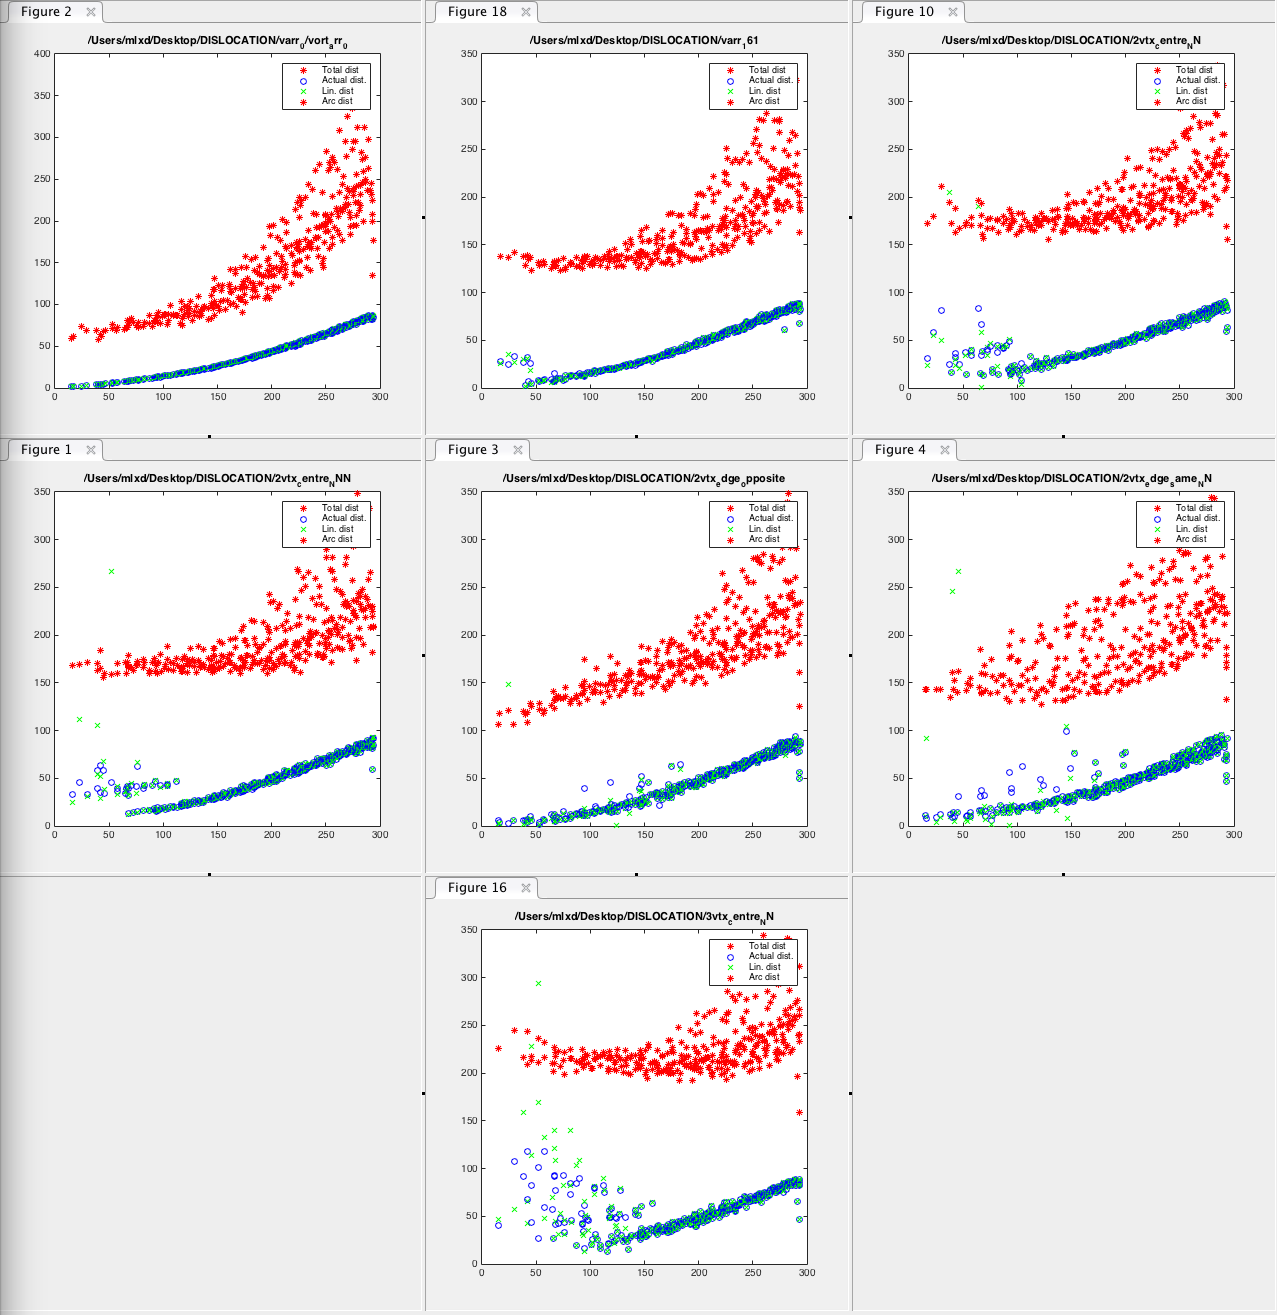
\includegraphics[width=0.5\textwidth]{ch6_phasegineer/imgs/vtx_distance_travelled}
    \caption{The length of the vortex tails following a set of different perturbations are given and comapred for different metrics. As expected, the greater the disturbance, the further the length travelled by the resulting lattice.}\label{fig:vtx_dist_travelled}
\end{figure}

\begin{figure}\centering
    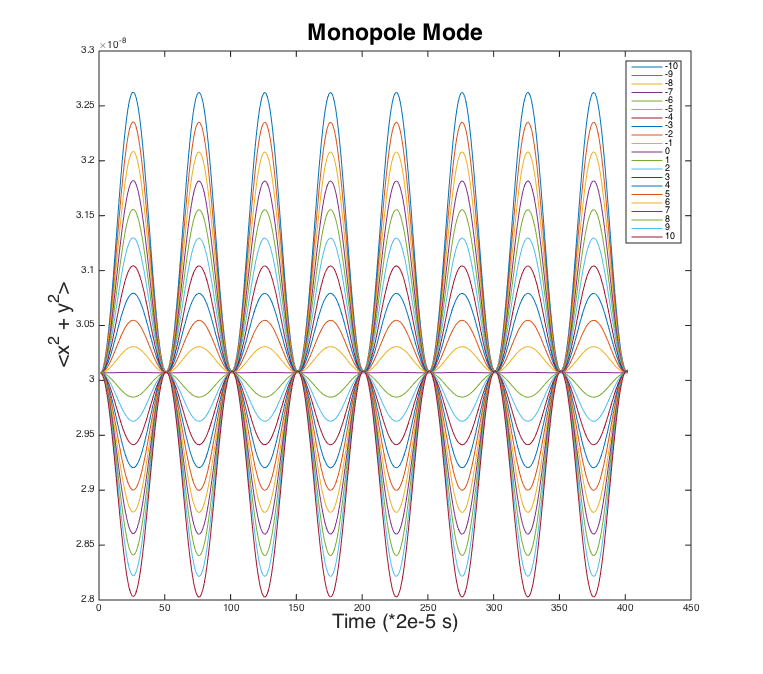
\includegraphics[width=0.5\textwidth]{ch6_phasegineer/imgs/mono}
    \caption{Monopole mode of the condensate following a different charged vortex imprint. A step-like increase or decrease in oscillation amplitude can be observed.}\label{fig:monopoles}
\end{figure}

\begin{figure}\centering
    \includegraphics[]{}
    \caption{}\label{}
\end{figure}

\begin{figure}\centering
    \includegraphics[]{}
    \caption{}\label{}
\end{figure}

\begin{figure}\centering
    \includegraphics[]{}
    \caption{}\label{}
\end{figure}

\begin{figure}\centering
    \includegraphics[]{}
    \caption{}\label{}
\end{figure}

\begin{figure}\centering
    \includegraphics[]{}
    \caption{}\label{}
\end{figure}
